\subsection{Cut Based Analysis}

\subsubsection{\mHi=115 \GeVcc\ analysis}

%%%%%%%%
\begin{figure}[!hbtp]
\begin{center}
\subfigure[]{\label{subfig:mh115_0j_cut_of_mll}
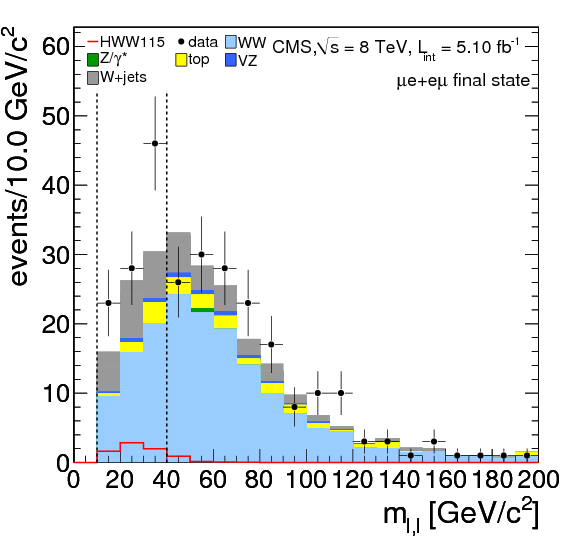
\includegraphics[width=.38\textwidth]{figures/dilepmass_mh115_nj0_of.png}}
\subfigure[]{\label{subfig:mh115_0j_cut_of_dphi}
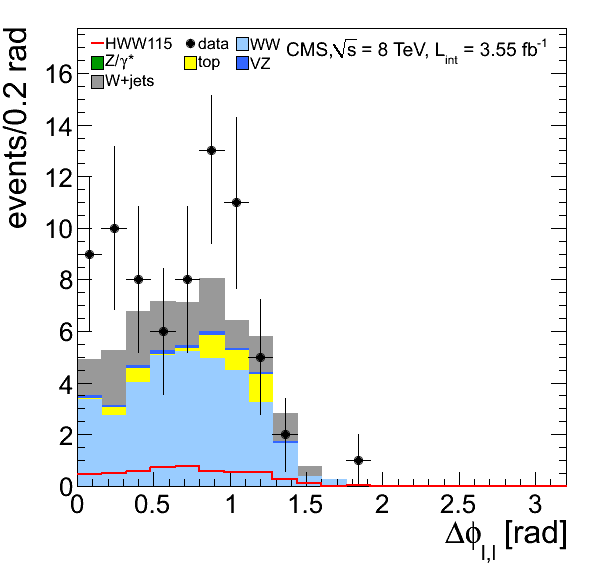
\includegraphics[width=.38\textwidth]{figures/dPhi_mh115_nj0_of.png}}\\
\subfigure[]{\label{subfig:mh115_0j_cut_of_mt}
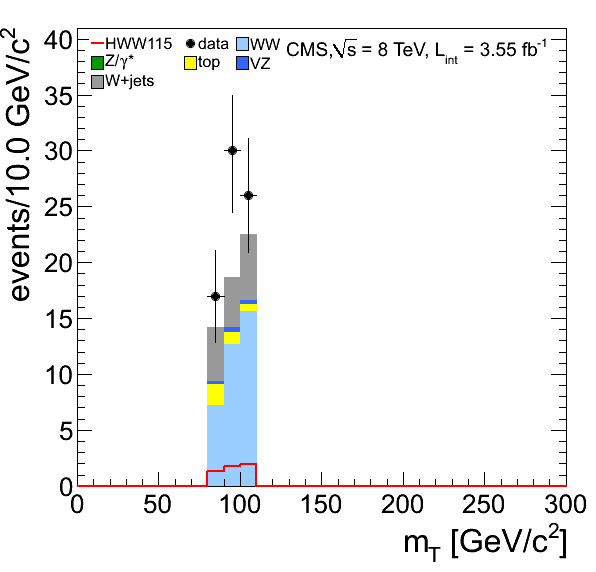
\includegraphics[width=.38\textwidth]{figures/mt_mh115_nj0_of.png}}
\subfigure[]{\label{subfig:mh115_0j_cut_of_ptll}
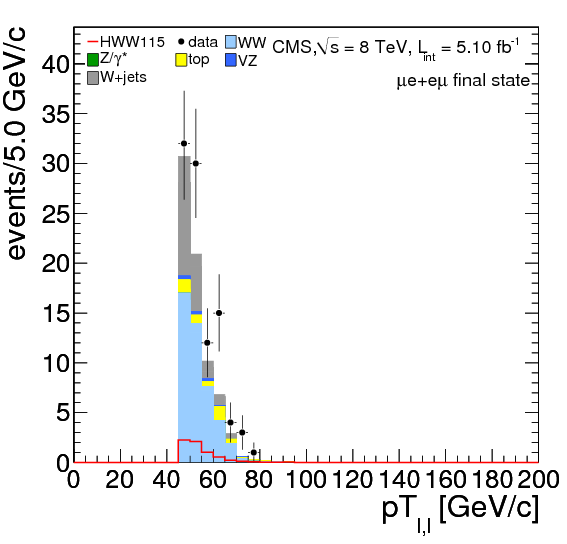
\includegraphics[width=.38\textwidth]{figures/dileppt_mh115_nj0_of.png}}\\
\subfigure[]{\label{subfig:mh115_0j_cut_of_ptl1}
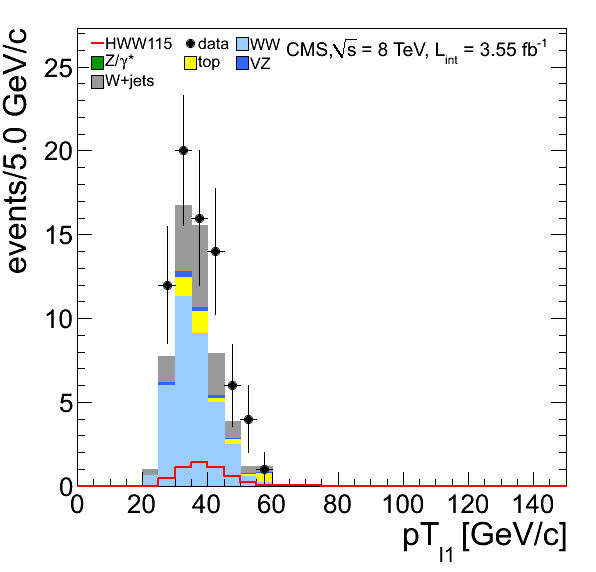
\includegraphics[width=.38\textwidth]{figures/lep1pt_mh115_nj0_of.png}}
\subfigure[]{\label{subfig:mh115_0j_cut_of_ptl2}
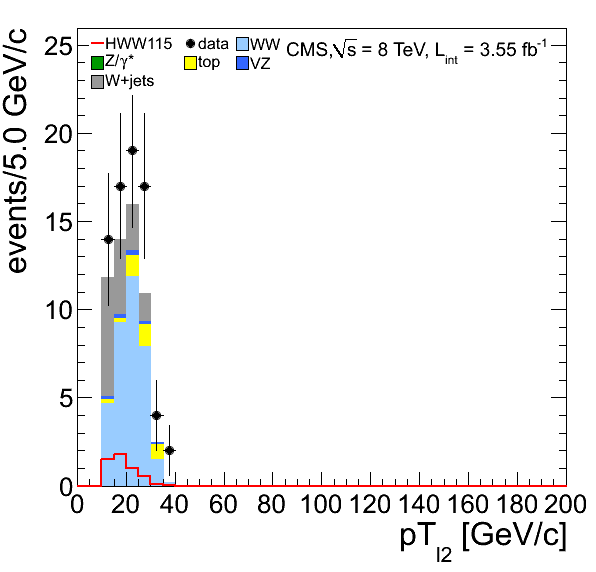
\includegraphics[width=.38\textwidth]{figures/lep2pt_mh115_nj0_of.png}}\\
\caption{Distribution of main kinematic variables after OF cut based analysis for \mHi=115 \GeVcc\ in the 0-jet bin.}
\label{fig:mh115_0j_cut_of}
\end{center}
\end{figure}
%%%%%%%%
\clearpage
%%%%%%%%
\begin{figure}[!hbtp]
\begin{center}
\subfigure[]{\label{subfig:mh115_0j_cut_sf_mll}
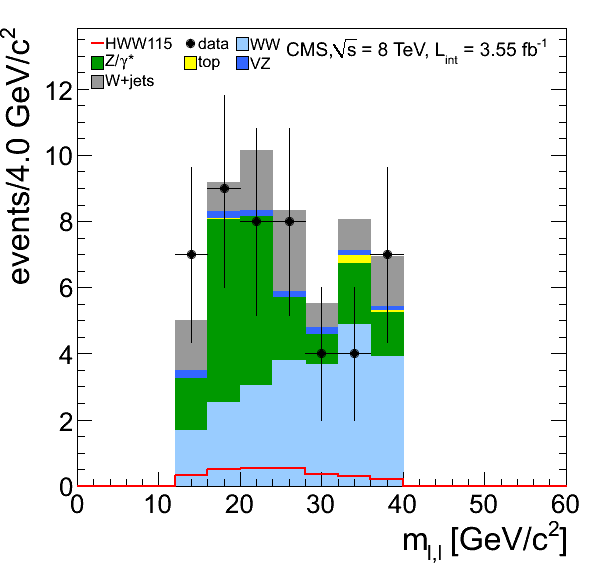
\includegraphics[width=.38\textwidth]{figures/dilepmass_mh115_nj0_sf.png}}
\subfigure[]{\label{subfig:mh115_0j_cut_sf_dphi}
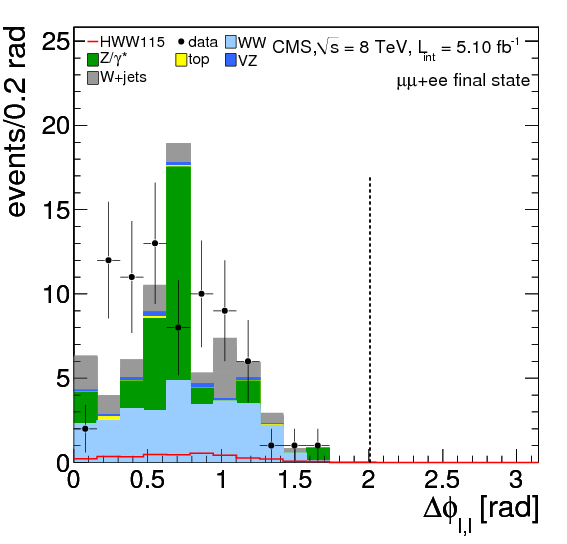
\includegraphics[width=.38\textwidth]{figures/dPhi_mh115_nj0_sf.png}}\\
\subfigure[]{\label{subfig:mh115_0j_cut_sf_mt}
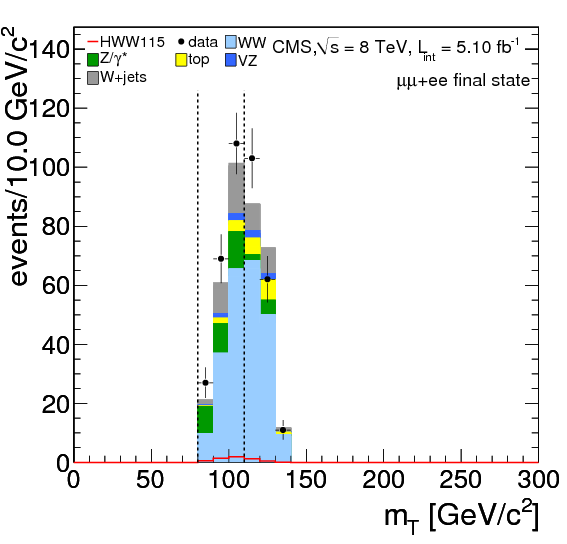
\includegraphics[width=.38\textwidth]{figures/mt_mh115_nj0_sf.png}}
\subfigure[]{\label{subfig:mh115_0j_cut_sf_ptll}
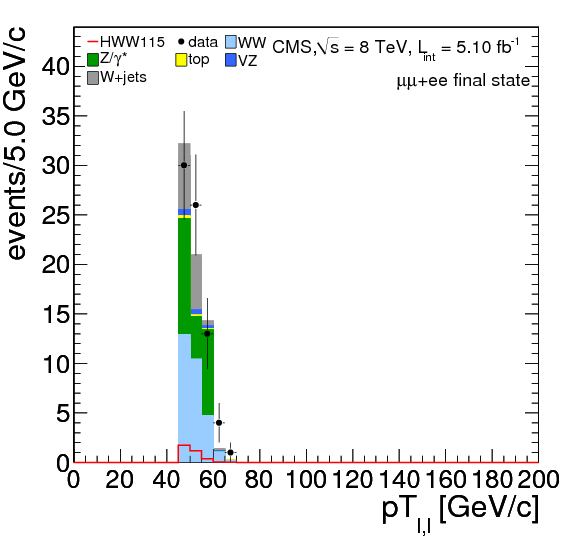
\includegraphics[width=.38\textwidth]{figures/dileppt_mh115_nj0_sf.png}}\\
\subfigure[]{\label{subfig:mh115_0j_cut_sf_ptl1}
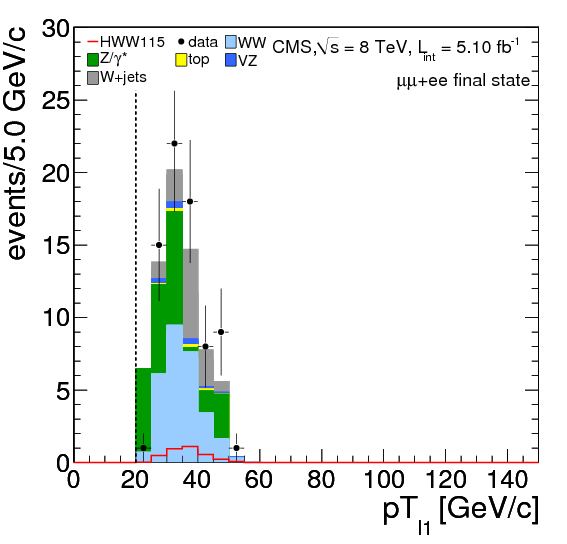
\includegraphics[width=.38\textwidth]{figures/lep1pt_mh115_nj0_sf.png}}
\subfigure[]{\label{subfig:mh115_0j_cut_sf_ptl2}
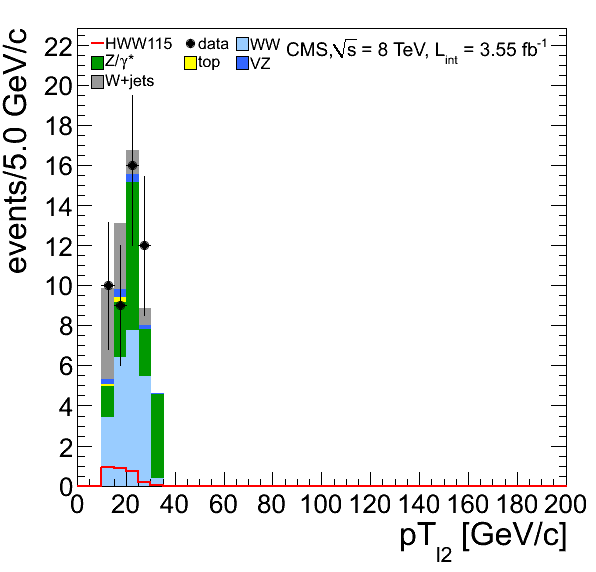
\includegraphics[width=.38\textwidth]{figures/lep2pt_mh115_nj0_sf.png}}\\
\caption{Distribution sf main kinematic variables after SF cut based analysis for \mHi=115 \GeVcc\ in the 0-jet bin.}
\label{fig:mh115_0j_cut_sf}
\end{center}
\end{figure}
%%%%%%%%
\clearpage
%%%%%%%%
\begin{figure}[!hbtp]
\begin{center}
\subfigure[]{\label{subfig:mh115_1j_cut_of_mll}
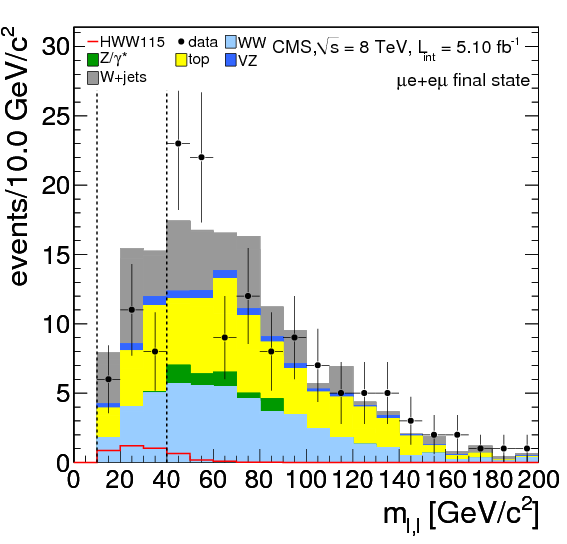
\includegraphics[width=.38\textwidth]{figures/dilepmass_mh115_nj1_of.png}}
\subfigure[]{\label{subfig:mh115_1j_cut_of_dphi}
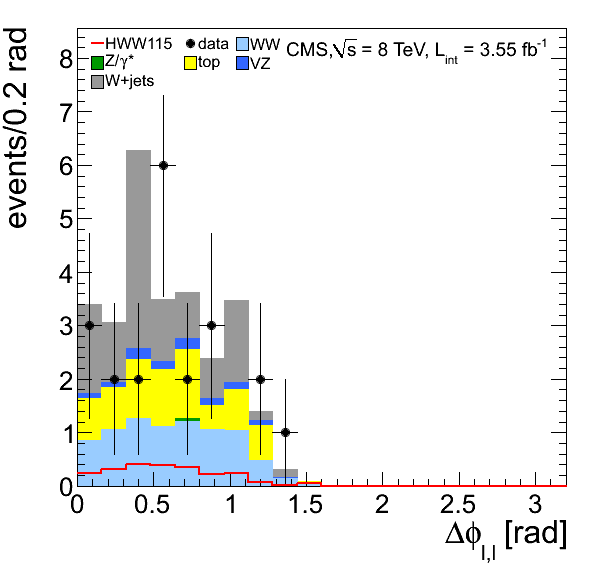
\includegraphics[width=.38\textwidth]{figures/dPhi_mh115_nj1_of.png}}\\
\subfigure[]{\label{subfig:mh115_1j_cut_of_mt}
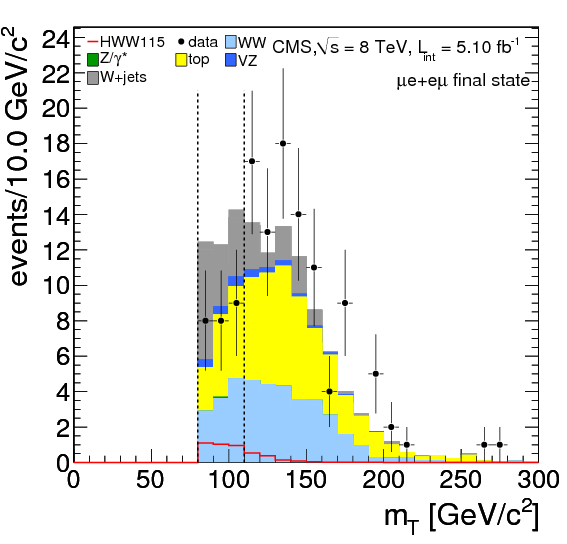
\includegraphics[width=.38\textwidth]{figures/mt_mh115_nj1_of.png}}
\subfigure[]{\label{subfig:mh115_1j_cut_of_ptll}
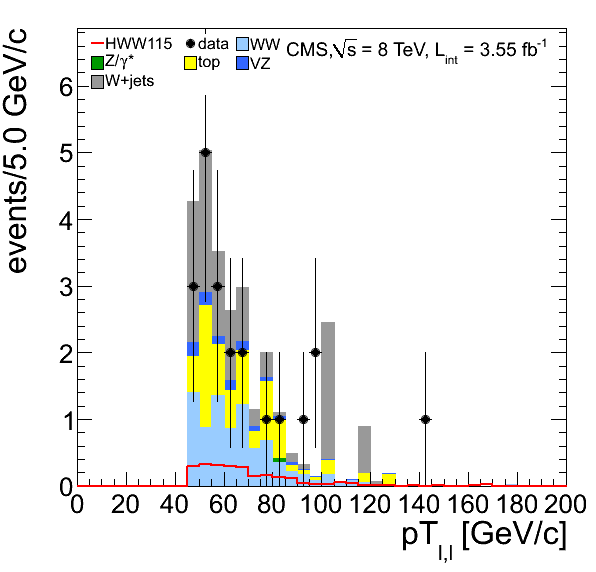
\includegraphics[width=.38\textwidth]{figures/dileppt_mh115_nj1_of.png}}\\
\subfigure[]{\label{subfig:mh115_1j_cut_of_ptl1}
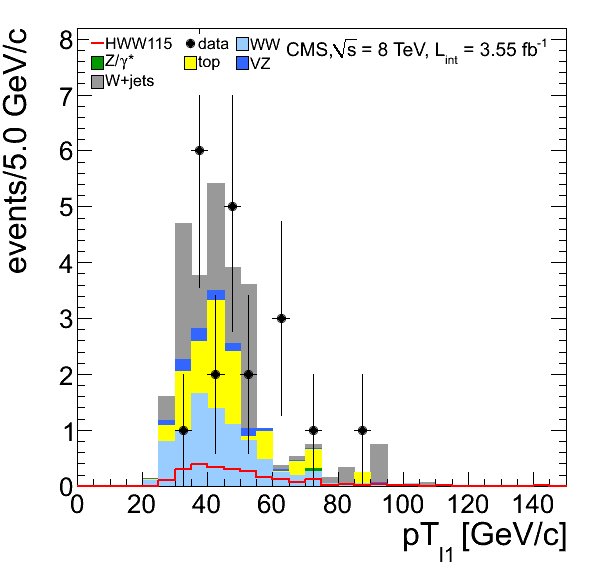
\includegraphics[width=.38\textwidth]{figures/lep1pt_mh115_nj1_of.png}}
\subfigure[]{\label{subfig:mh115_1j_cut_of_ptl2}
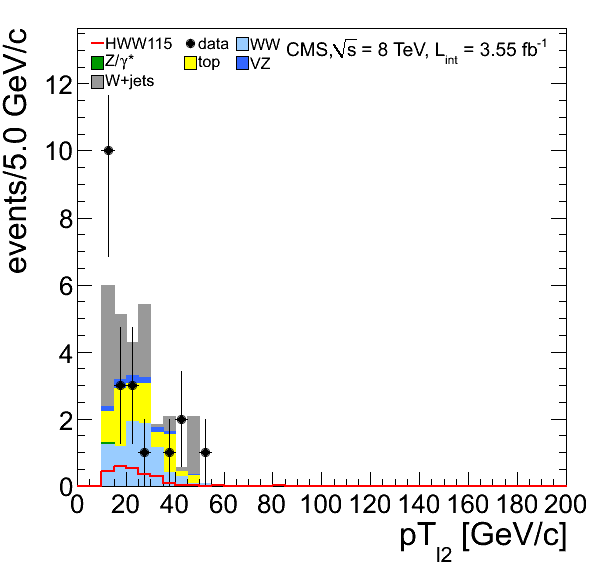
\includegraphics[width=.38\textwidth]{figures/lep2pt_mh115_nj1_of.png}}\\
\caption{Distribution of main kinematic variables after OF cut based analysis for \mHi=115 \GeVcc\ in the 1-jet bin.}
\label{fig:mh115_1j_cut_of}
\end{center}
\end{figure}
%%%%%%%%
\clearpage
%%%%%%%%
\begin{figure}[!hbtp]
\begin{center}
\subfigure[]{\label{subfig:mh115_1j_cut_sf_mll}
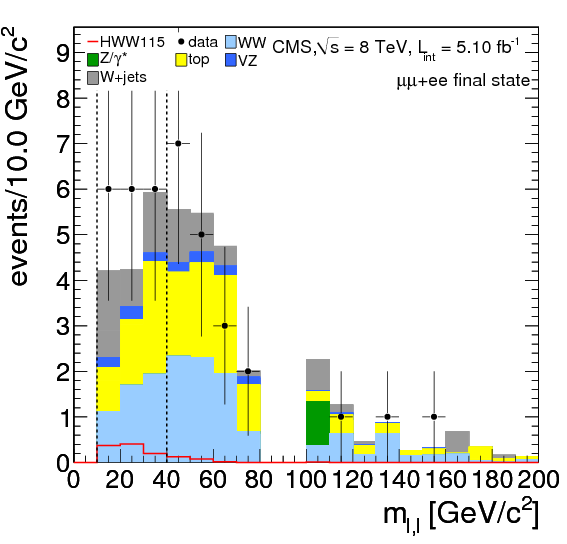
\includegraphics[width=.38\textwidth]{figures/dilepmass_mh115_nj1_sf.png}}
\subfigure[]{\label{subfig:mh115_1j_cut_sf_dphi}
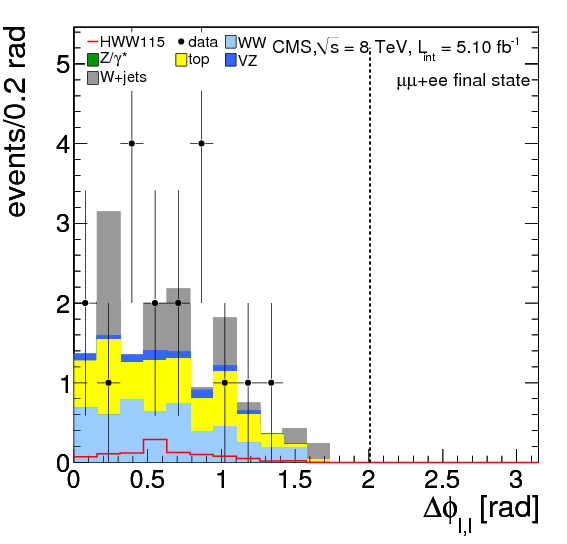
\includegraphics[width=.38\textwidth]{figures/dPhi_mh115_nj1_sf.png}}\\
\subfigure[]{\label{subfig:mh115_1j_cut_sf_mt}
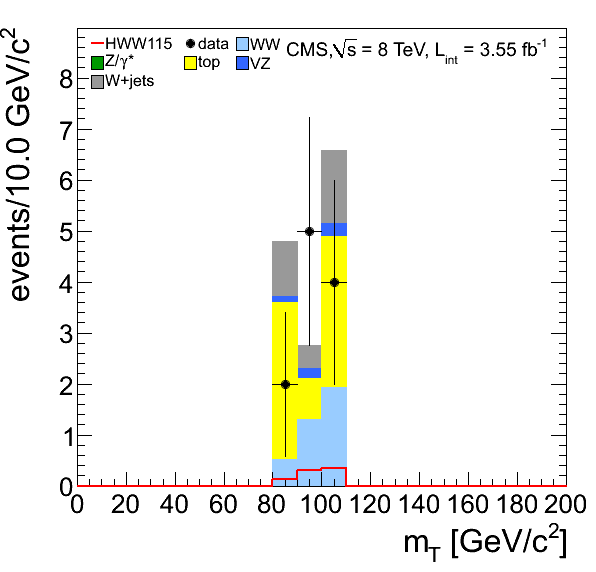
\includegraphics[width=.38\textwidth]{figures/mt_mh115_nj1_sf.png}}
\subfigure[]{\label{subfig:mh115_1j_cut_sf_ptll}
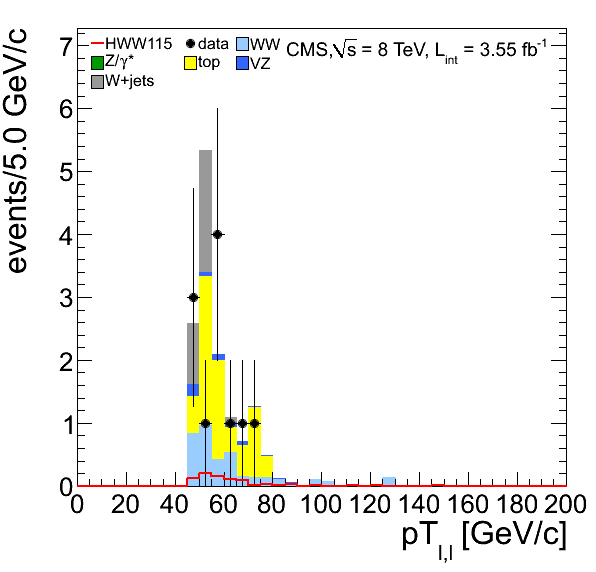
\includegraphics[width=.38\textwidth]{figures/dileppt_mh115_nj1_sf.png}}\\
\subfigure[]{\label{subfig:mh115_1j_cut_sf_ptl1}
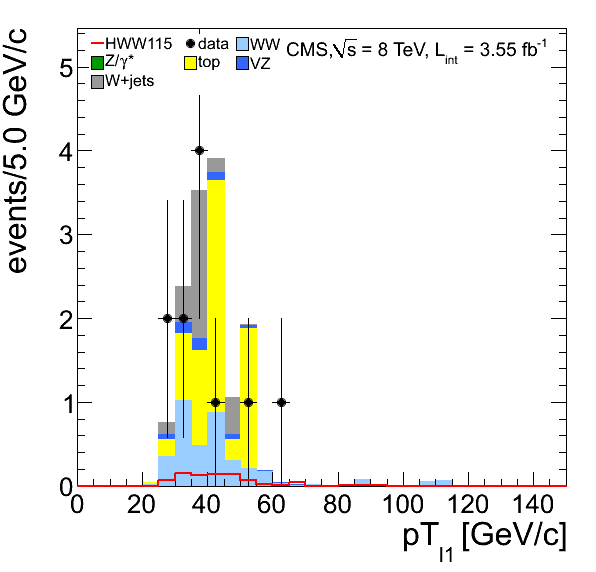
\includegraphics[width=.38\textwidth]{figures/lep1pt_mh115_nj1_sf.png}}
\subfigure[]{\label{subfig:mh115_1j_cut_sf_ptl2}
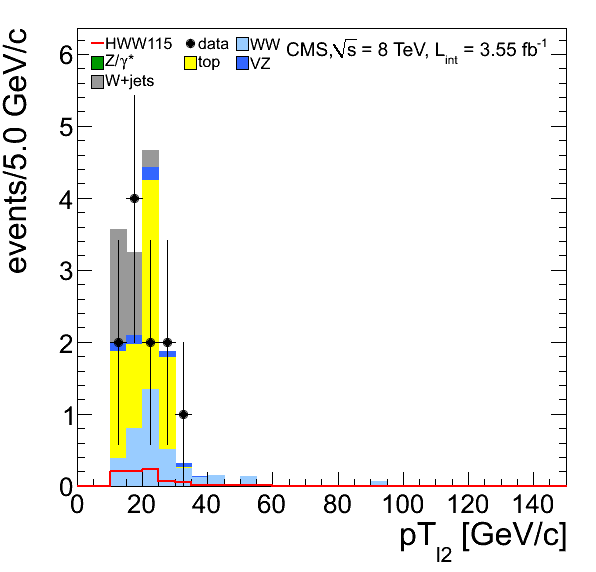
\includegraphics[width=.38\textwidth]{figures/lep2pt_mh115_nj1_sf.png}}\\
\caption{Distribution sf main kinematic variables after SF cut based analysis for \mHi=115 \GeVcc\ in the 1-jet bin.
The Zjets contribution is missing since no MC events survive after full selection.}
\label{fig:mh115_1j_cut_sf}
\end{center}
\end{figure}
%%%%%%%%
\clearpage
%%%%%%%%
\begin{figure}[!hbtp]
\begin{center}
\subfigure[]{\label{subfig:mh115_2j_cut_of_mll}
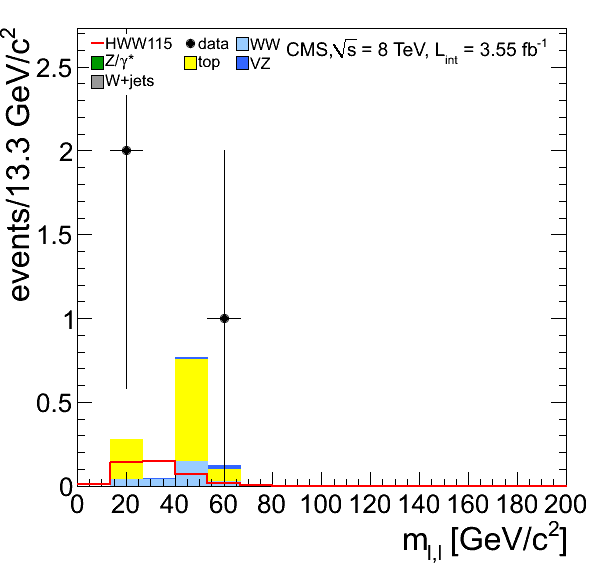
\includegraphics[width=.38\textwidth]{figures/dilepmass_mh115_nj2_of.png}}
\subfigure[]{\label{subfig:mh115_2j_cut_of_dphi}
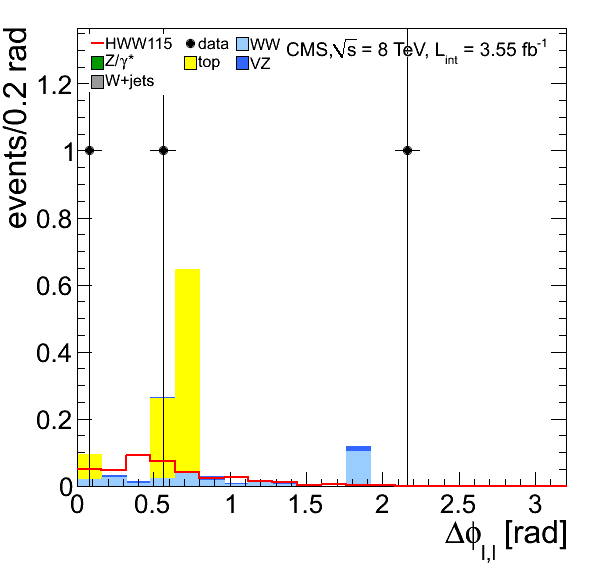
\includegraphics[width=.38\textwidth]{figures/dPhi_mh115_nj2_of.png}}\\
\subfigure[]{\label{subfig:mh115_2j_cut_of_mt}
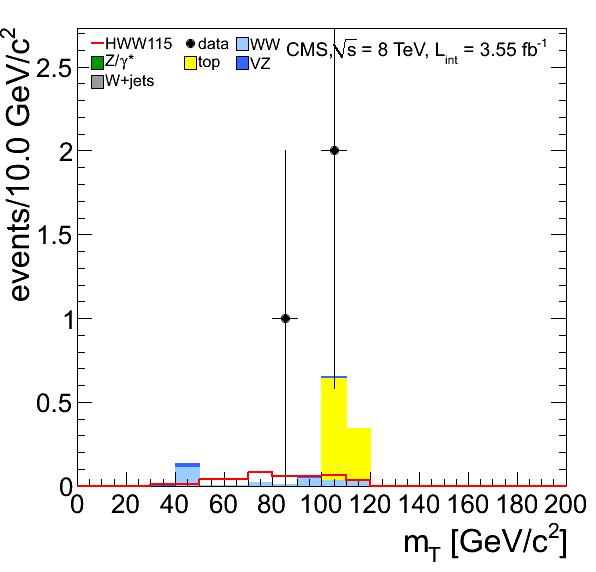
\includegraphics[width=.38\textwidth]{figures/mt_mh115_nj2_of.png}}
\subfigure[]{\label{subfig:mh115_2j_cut_of_ptll}
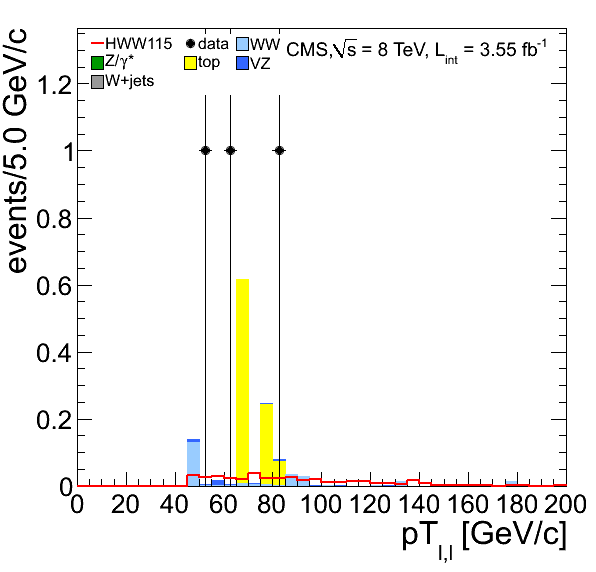
\includegraphics[width=.38\textwidth]{figures/dileppt_mh115_nj2_of.png}}\\
\subfigure[]{\label{subfig:mh115_2j_cut_of_ptl1}
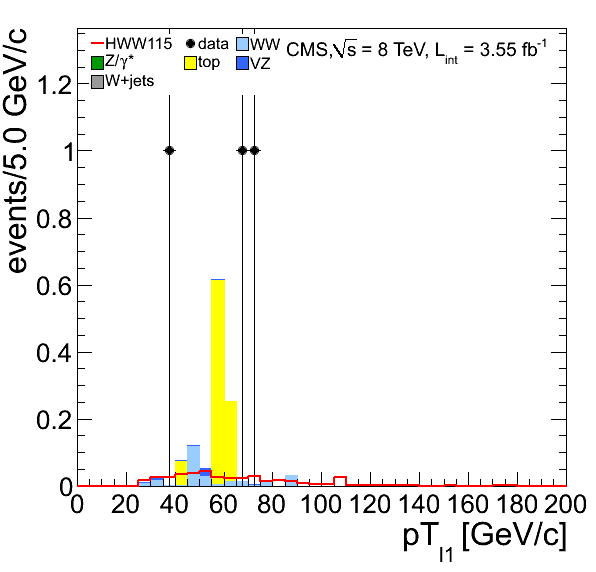
\includegraphics[width=.38\textwidth]{figures/lep1pt_mh115_nj2_of.png}}
\subfigure[]{\label{subfig:mh115_2j_cut_of_ptl2}
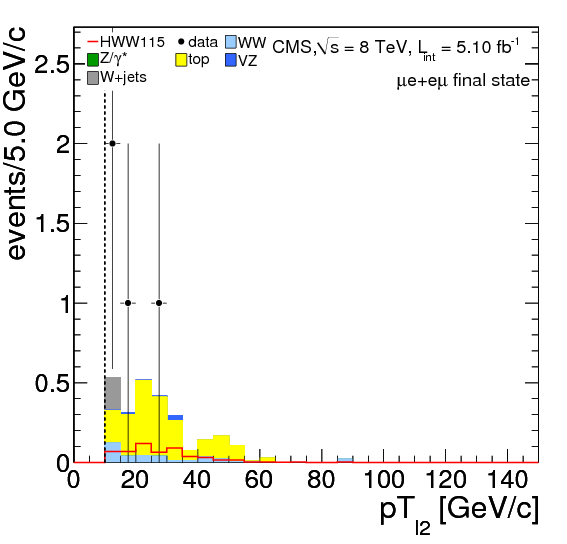
\includegraphics[width=.38\textwidth]{figures/lep2pt_mh115_nj2_of.png}}\\
\caption{Distribution of main kinematic variables after OF cut based analysis for \mHi=115 \GeVcc\ in the VBF channel.}
\label{fig:mh115_2j_cut_of}
\end{center}
\end{figure}
%%%%%%%%
\clearpage
%%%%%%%%
\begin{figure}[!hbtp]
\begin{center}
\subfigure[]{\label{subfig:mh115_2j_cut_sf_mll}
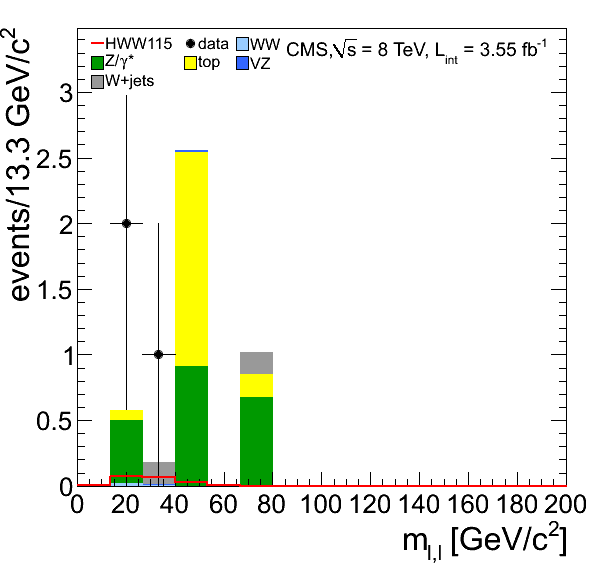
\includegraphics[width=.38\textwidth]{figures/dilepmass_mh115_nj2_sf.png}}
\subfigure[]{\label{subfig:mh115_2j_cut_sf_dphi}
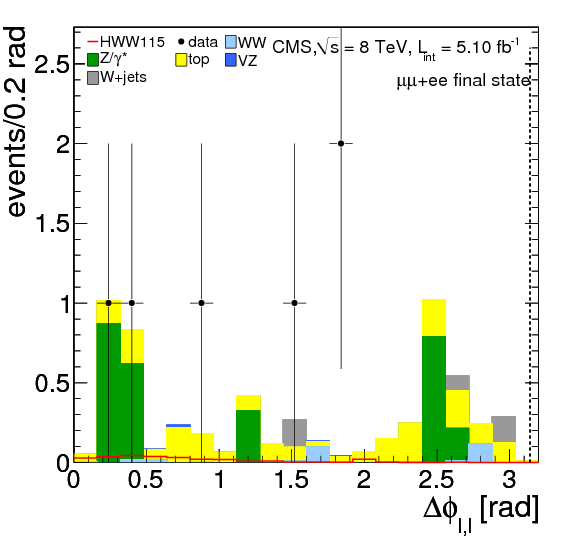
\includegraphics[width=.38\textwidth]{figures/dPhi_mh115_nj2_sf.png}}\\
\subfigure[]{\label{subfig:mh115_2j_cut_sf_mt}
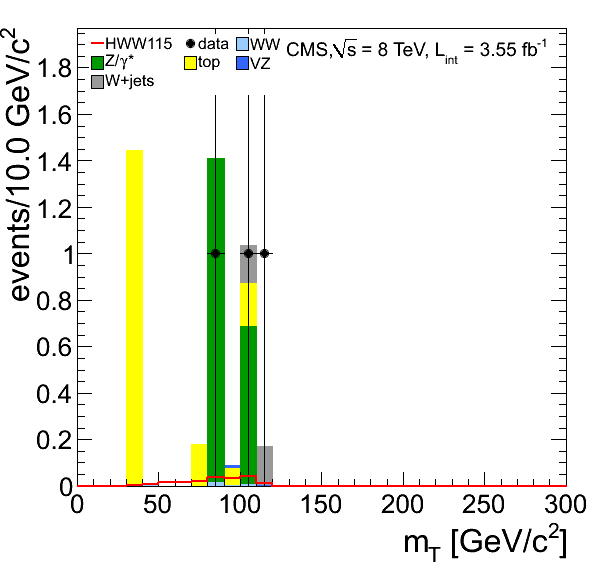
\includegraphics[width=.38\textwidth]{figures/mt_mh115_nj2_sf.png}}
\subfigure[]{\label{subfig:mh115_2j_cut_sf_ptll}
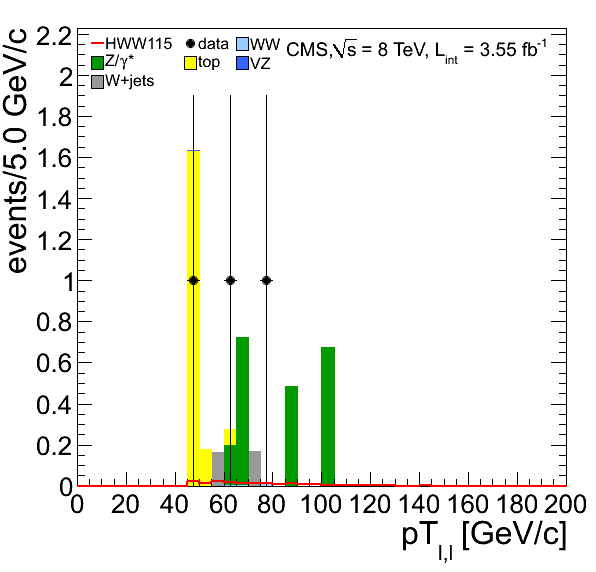
\includegraphics[width=.38\textwidth]{figures/dileppt_mh115_nj2_sf.png}}\\
\subfigure[]{\label{subfig:mh115_2j_cut_sf_ptl1}
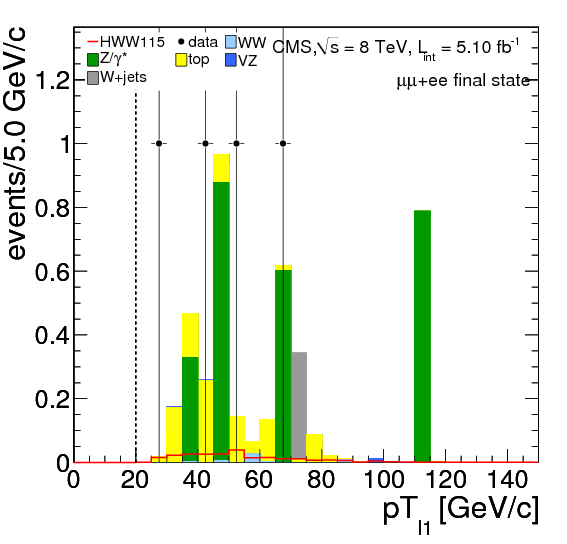
\includegraphics[width=.38\textwidth]{figures/lep1pt_mh115_nj2_sf.png}}
\subfigure[]{\label{subfig:mh115_2j_cut_sf_ptl2}
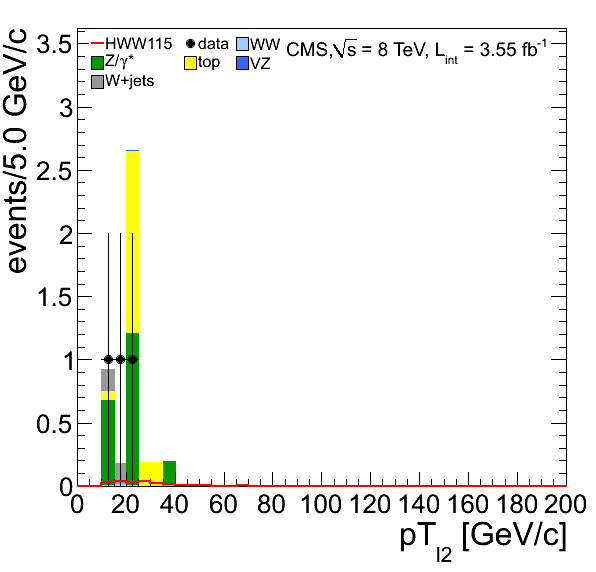
\includegraphics[width=.38\textwidth]{figures/lep2pt_mh115_nj2_sf.png}}\\
\caption{Distribution sf main kinematic variables after SF cut based analysis for \mHi=115 \GeVcc\ in the VBF channel.}
\label{fig:mh115_2j_cut_sf}
\end{center}
\end{figure}
%%%%%%%%
\clearpage


\subsubsection{\mHi=120 \GeVcc\ analysis}

%%%%%%%%
\begin{figure}[!hbtp]
\begin{center}
\subfigure[]{\label{subfig:mh120_0j_cut_of_mll}
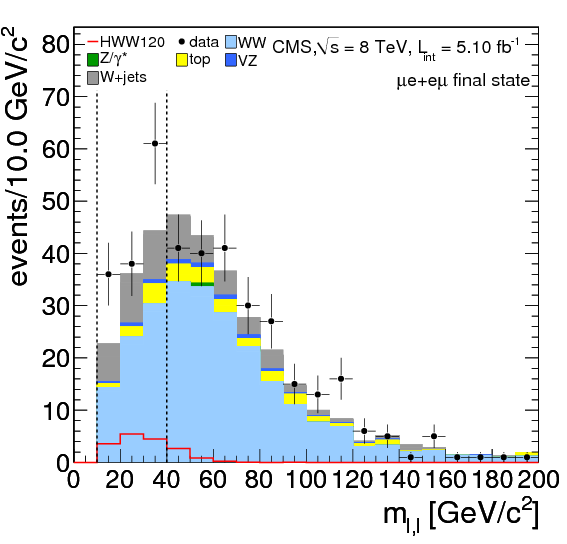
\includegraphics[width=.38\textwidth]{figures/dilepmass_mh120_nj0_of.png}}
\subfigure[]{\label{subfig:mh120_0j_cut_of_dphi}
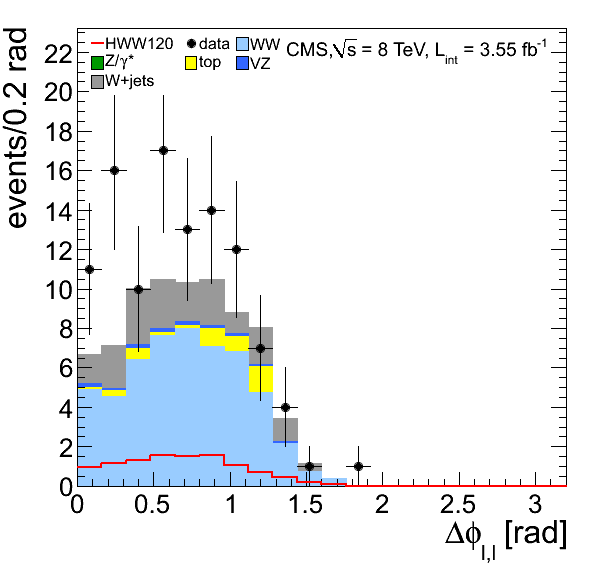
\includegraphics[width=.38\textwidth]{figures/dPhi_mh120_nj0_of.png}}\\
\subfigure[]{\label{subfig:mh120_0j_cut_of_mt}
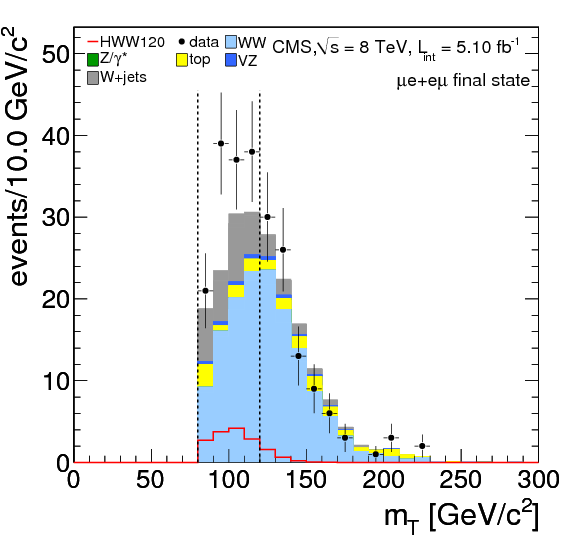
\includegraphics[width=.38\textwidth]{figures/mt_mh120_nj0_of.png}}
\subfigure[]{\label{subfig:mh120_0j_cut_of_ptll}
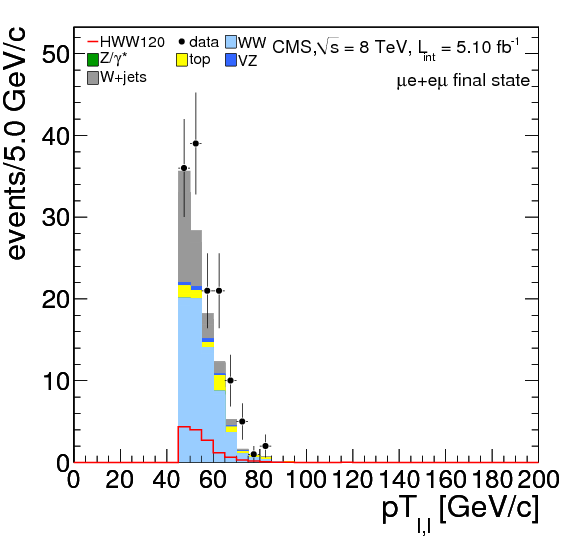
\includegraphics[width=.38\textwidth]{figures/dileppt_mh120_nj0_of.png}}\\
\subfigure[]{\label{subfig:mh120_0j_cut_of_ptl1}
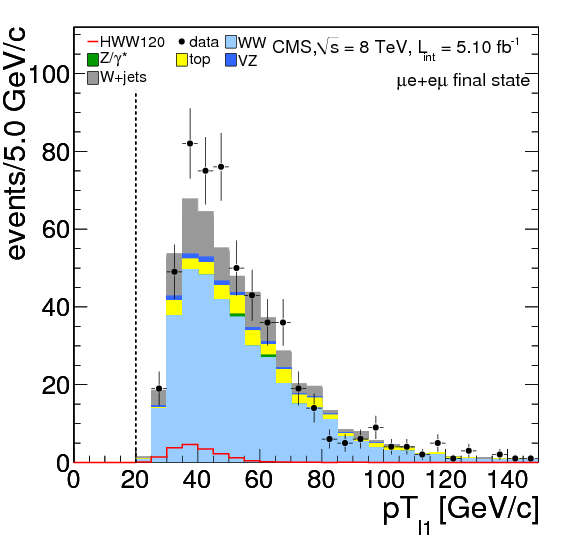
\includegraphics[width=.38\textwidth]{figures/lep1pt_mh120_nj0_of.png}}
\subfigure[]{\label{subfig:mh120_0j_cut_of_ptl2}
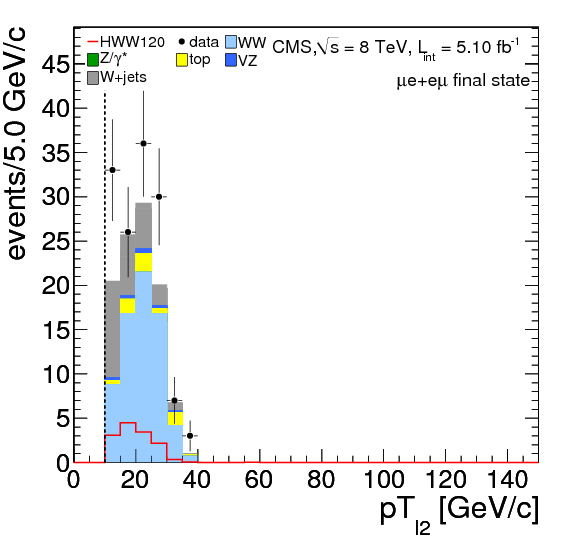
\includegraphics[width=.38\textwidth]{figures/lep2pt_mh120_nj0_of.png}}\\
\caption{Distribution of main kinematic variables after OF cut based analysis for \mHi=120 \GeVcc\ in the 0-jet bin.}
\label{fig:mh120_0j_cut_of}
\end{center}
\end{figure}
%%%%%%%%
\clearpage
%%%%%%%%
\begin{figure}[!hbtp]
\begin{center}
\subfigure[]{\label{subfig:mh120_0j_cut_sf_mll}
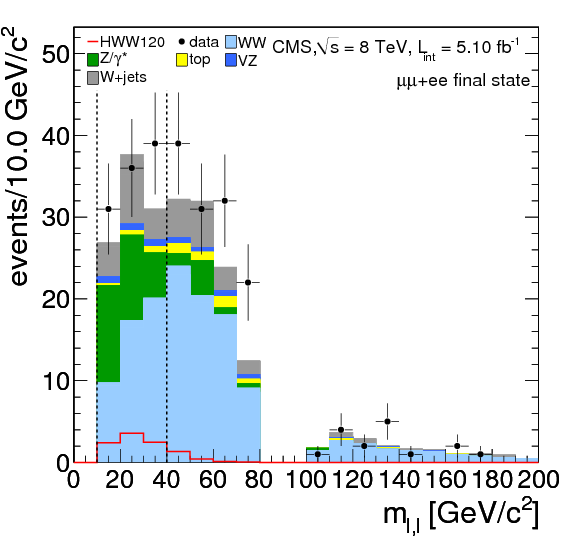
\includegraphics[width=.38\textwidth]{figures/dilepmass_mh120_nj0_sf.png}}
\subfigure[]{\label{subfig:mh120_0j_cut_sf_dphi}
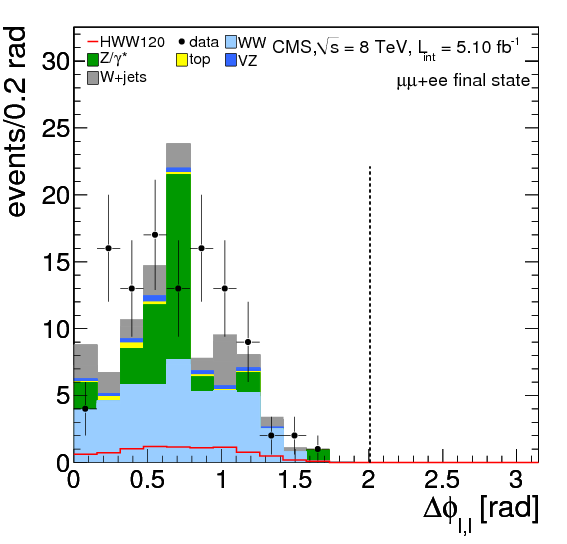
\includegraphics[width=.38\textwidth]{figures/dPhi_mh120_nj0_sf.png}}\\
\subfigure[]{\label{subfig:mh120_0j_cut_sf_mt}
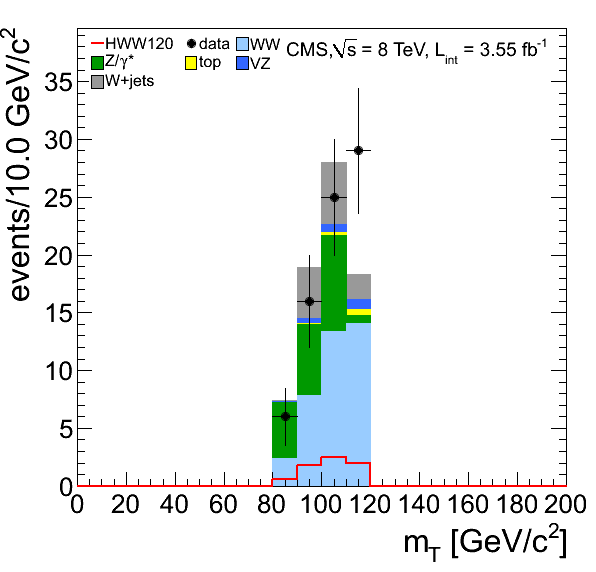
\includegraphics[width=.38\textwidth]{figures/mt_mh120_nj0_sf.png}}
\subfigure[]{\label{subfig:mh120_0j_cut_sf_ptll}
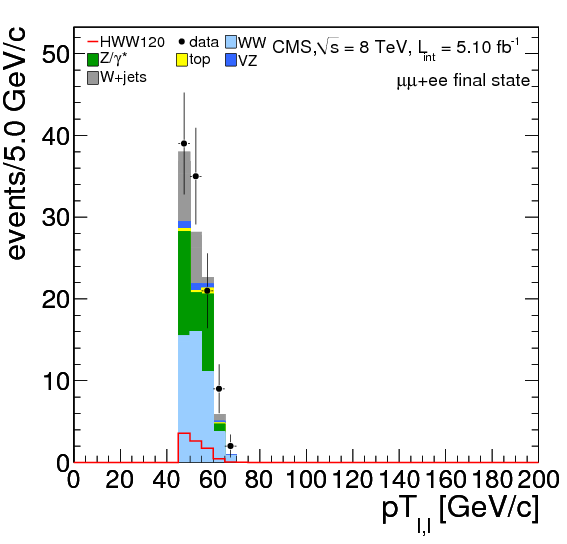
\includegraphics[width=.38\textwidth]{figures/dileppt_mh120_nj0_sf.png}}\\
\subfigure[]{\label{subfig:mh120_0j_cut_sf_ptl1}
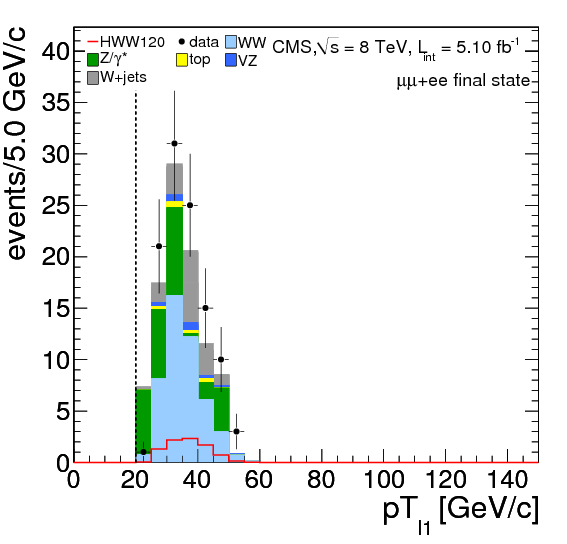
\includegraphics[width=.38\textwidth]{figures/lep1pt_mh120_nj0_sf.png}}
\subfigure[]{\label{subfig:mh120_0j_cut_sf_ptl2}
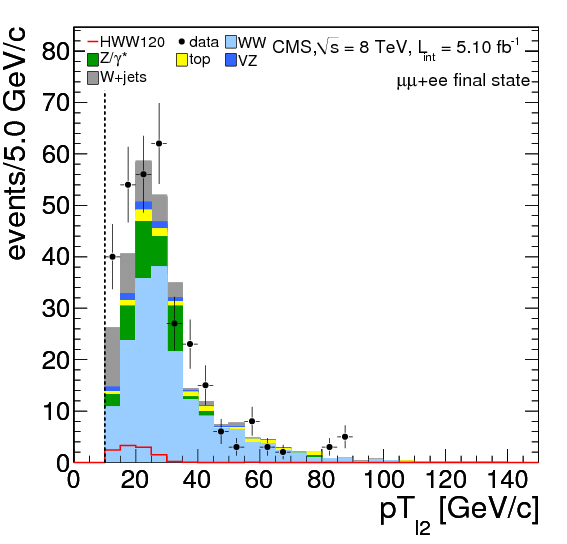
\includegraphics[width=.38\textwidth]{figures/lep2pt_mh120_nj0_sf.png}}\\
\caption{Distribution sf main kinematic variables after SF cut based analysis for \mHi=120 \GeVcc\ in the 0-jet bin.}
\label{fig:mh120_0j_cut_sf}
\end{center}
\end{figure}
%%%%%%%%
\clearpage
%%%%%%%%
\begin{figure}[!hbtp]
\begin{center}
\subfigure[]{\label{subfig:mh120_1j_cut_of_mll}
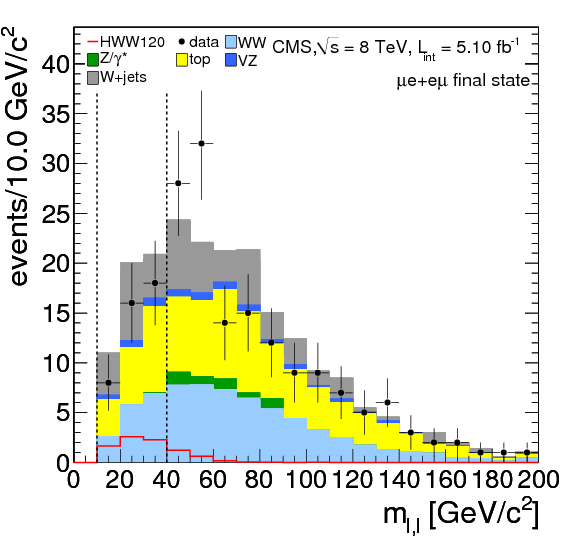
\includegraphics[width=.38\textwidth]{figures/dilepmass_mh120_nj1_of.png}}
\subfigure[]{\label{subfig:mh120_1j_cut_of_dphi}
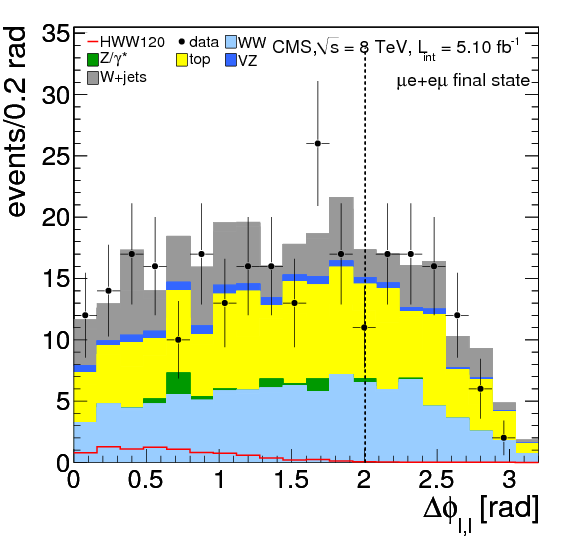
\includegraphics[width=.38\textwidth]{figures/dPhi_mh120_nj1_of.png}}\\
\subfigure[]{\label{subfig:mh120_1j_cut_of_mt}
\includegraphics[width=.38\textwidth]{figures/mt_mh120_nj1_of.png}}
\subfigure[]{\label{subfig:mh120_1j_cut_of_ptll}
\includegraphics[width=.38\textwidth]{figures/dileppt_mh120_nj1_of.png}}\\
\subfigure[]{\label{subfig:mh120_1j_cut_of_ptl1}
\includegraphics[width=.38\textwidth]{figures/lep1pt_mh120_nj1_of.png}}
\subfigure[]{\label{subfig:mh120_1j_cut_of_ptl2}
\includegraphics[width=.38\textwidth]{figures/lep2pt_mh120_nj1_of.png}}\\
\caption{Distribution of main kinematic variables after OF cut based analysis for \mHi=120 \GeVcc\ in the 1-jet bin.}
\label{fig:mh120_1j_cut_of}
\end{center}
\end{figure}
%%%%%%%%
\clearpage
%%%%%%%%
\begin{figure}[!hbtp]
\begin{center}
\subfigure[]{\label{subfig:mh120_1j_cut_sf_mll}
\includegraphics[width=.38\textwidth]{figures/dilepmass_mh120_nj1_sf.png}}
\subfigure[]{\label{subfig:mh120_1j_cut_sf_dphi}
\includegraphics[width=.38\textwidth]{figures/dPhi_mh120_nj1_sf.png}}\\
\subfigure[]{\label{subfig:mh120_1j_cut_sf_mt}
\includegraphics[width=.38\textwidth]{figures/mt_mh120_nj1_sf.png}}
\subfigure[]{\label{subfig:mh120_1j_cut_sf_ptll}
\includegraphics[width=.38\textwidth]{figures/dileppt_mh120_nj1_sf.png}}\\
\subfigure[]{\label{subfig:mh120_1j_cut_sf_ptl1}
\includegraphics[width=.38\textwidth]{figures/lep1pt_mh120_nj1_sf.png}}
\subfigure[]{\label{subfig:mh120_1j_cut_sf_ptl2}
\includegraphics[width=.38\textwidth]{figures/lep2pt_mh120_nj1_sf.png}}\\
\caption{Distribution sf main kinematic variables after SF cut based analysis for \mHi=120 \GeVcc\ in the 1-jet bin.
The Zjets contribution is missing since no MC events survive after full selection.}
\label{fig:mh120_1j_cut_sf}
\end{center}
\end{figure}
%%%%%%%%
\clearpage
%%%%%%%%
\begin{figure}[!hbtp]
\begin{center}
\subfigure[]{\label{subfig:mh120_2j_cut_of_mll}
\includegraphics[width=.38\textwidth]{figures/dilepmass_mh120_nj2_of.png}}
\subfigure[]{\label{subfig:mh120_2j_cut_of_dphi}
\includegraphics[width=.38\textwidth]{figures/dPhi_mh120_nj2_of.png}}\\
\subfigure[]{\label{subfig:mh120_2j_cut_of_mt}
\includegraphics[width=.38\textwidth]{figures/mt_mh120_nj2_of.png}}
\subfigure[]{\label{subfig:mh120_2j_cut_of_ptll}
\includegraphics[width=.38\textwidth]{figures/dileppt_mh120_nj2_of.png}}\\
\subfigure[]{\label{subfig:mh120_2j_cut_of_ptl1}
\includegraphics[width=.38\textwidth]{figures/lep1pt_mh120_nj2_of.png}}
\subfigure[]{\label{subfig:mh120_2j_cut_of_ptl2}
\includegraphics[width=.38\textwidth]{figures/lep2pt_mh120_nj2_of.png}}\\
\caption{Distribution of main kinematic variables after OF cut based analysis for \mHi=120 \GeVcc\ in the VBF channel.}
\label{fig:mh120_2j_cut_of}
\end{center}
\end{figure}
%%%%%%%%
\clearpage
%%%%%%%%
\begin{figure}[!hbtp]
\begin{center}
\subfigure[]{\label{subfig:mh120_2j_cut_sf_mll}
\includegraphics[width=.38\textwidth]{figures/dilepmass_mh120_nj2_sf.png}}
\subfigure[]{\label{subfig:mh120_2j_cut_sf_dphi}
\includegraphics[width=.38\textwidth]{figures/dPhi_mh120_nj2_sf.png}}\\
\subfigure[]{\label{subfig:mh120_2j_cut_sf_mt}
\includegraphics[width=.38\textwidth]{figures/mt_mh120_nj2_sf.png}}
\subfigure[]{\label{subfig:mh120_2j_cut_sf_ptll}
\includegraphics[width=.38\textwidth]{figures/dileppt_mh120_nj2_sf.png}}\\
\subfigure[]{\label{subfig:mh120_2j_cut_sf_ptl1}
\includegraphics[width=.38\textwidth]{figures/lep1pt_mh120_nj2_sf.png}}
\subfigure[]{\label{subfig:mh120_2j_cut_sf_ptl2}
\includegraphics[width=.38\textwidth]{figures/lep2pt_mh120_nj2_sf.png}}\\
\caption{Distribution sf main kinematic variables after SF cut based analysis for \mHi=120 \GeVcc\ in the VBF channel.}
\label{fig:mh120_2j_cut_sf}
\end{center}
\end{figure}
%%%%%%%%
\clearpage


\subsubsection{\mHi=125 \GeVcc\ analysis}

%%%%%%%%
\begin{figure}[!hbtp]
\begin{center}
\subfigure[]{\label{subfig:mh125_0j_cut_of_mll}
\includegraphics[width=.38\textwidth]{figures/dilepmass_mh125_nj0_of.png}}
\subfigure[]{\label{subfig:mh125_0j_cut_of_dphi}
\includegraphics[width=.38\textwidth]{figures/dPhi_mh125_nj0_of.png}}\\
\subfigure[]{\label{subfig:mh125_0j_cut_of_mt}
\includegraphics[width=.38\textwidth]{figures/mt_mh125_nj0_of.png}}
\subfigure[]{\label{subfig:mh125_0j_cut_of_ptll}
\includegraphics[width=.38\textwidth]{figures/dileppt_mh125_nj0_of.png}}\\
\subfigure[]{\label{subfig:mh125_0j_cut_of_ptl1}
\includegraphics[width=.38\textwidth]{figures/lep1pt_mh125_nj0_of.png}}
\subfigure[]{\label{subfig:mh125_0j_cut_of_ptl2}
\includegraphics[width=.38\textwidth]{figures/lep2pt_mh125_nj0_of.png}}\\
\caption{Distribution of main kinematic variables after OF cut based analysis for \mHi=125 \GeVcc\ in the 0-jet bin.}
\label{fig:mh125_0j_cut_of}
\end{center}
\end{figure}
%%%%%%%%
\clearpage
%%%%%%%%
\begin{figure}[!hbtp]
\begin{center}
\subfigure[]{\label{subfig:mh125_0j_cut_sf_mll}
\includegraphics[width=.38\textwidth]{figures/dilepmass_mh125_nj0_sf.png}}
\subfigure[]{\label{subfig:mh125_0j_cut_sf_dphi}
\includegraphics[width=.38\textwidth]{figures/dPhi_mh125_nj0_sf.png}}\\
\subfigure[]{\label{subfig:mh125_0j_cut_sf_mt}
\includegraphics[width=.38\textwidth]{figures/mt_mh125_nj0_sf.png}}
\subfigure[]{\label{subfig:mh125_0j_cut_sf_ptll}
\includegraphics[width=.38\textwidth]{figures/dileppt_mh125_nj0_sf.png}}\\
\subfigure[]{\label{subfig:mh125_0j_cut_sf_ptl1}
\includegraphics[width=.38\textwidth]{figures/lep1pt_mh125_nj0_sf.png}}
\subfigure[]{\label{subfig:mh125_0j_cut_sf_ptl2}
\includegraphics[width=.38\textwidth]{figures/lep2pt_mh125_nj0_sf.png}}\\
\caption{Distribution sf main kinematic variables after SF cut based analysis for \mHi=125 \GeVcc\ in the 0-jet bin.}
\label{fig:mh125_0j_cut_sf}
\end{center}
\end{figure}
%%%%%%%%
\clearpage
%%%%%%%%
\begin{figure}[!hbtp]
\begin{center}
\subfigure[]{\label{subfig:mh125_1j_cut_of_mll}
\includegraphics[width=.38\textwidth]{figures/dilepmass_mh125_nj1_of.png}}
\subfigure[]{\label{subfig:mh125_1j_cut_of_dphi}
\includegraphics[width=.38\textwidth]{figures/dPhi_mh125_nj1_of.png}}\\
\subfigure[]{\label{subfig:mh125_1j_cut_of_mt}
\includegraphics[width=.38\textwidth]{figures/mt_mh125_nj1_of.png}}
\subfigure[]{\label{subfig:mh125_1j_cut_of_ptll}
\includegraphics[width=.38\textwidth]{figures/dileppt_mh125_nj1_of.png}}\\
\subfigure[]{\label{subfig:mh125_1j_cut_of_ptl1}
\includegraphics[width=.38\textwidth]{figures/lep1pt_mh125_nj1_of.png}}
\subfigure[]{\label{subfig:mh125_1j_cut_of_ptl2}
\includegraphics[width=.38\textwidth]{figures/lep2pt_mh125_nj1_of.png}}\\
\caption{Distribution of main kinematic variables after OF cut based analysis for \mHi=125 \GeVcc\ in the 1-jet bin.}
\label{fig:mh125_1j_cut_of}
\end{center}
\end{figure}
%%%%%%%%
\clearpage
%%%%%%%%
\begin{figure}[!hbtp]
\begin{center}
\subfigure[]{\label{subfig:mh125_1j_cut_sf_mll}
\includegraphics[width=.38\textwidth]{figures/dilepmass_mh125_nj1_sf.png}}
\subfigure[]{\label{subfig:mh125_1j_cut_sf_dphi}
\includegraphics[width=.38\textwidth]{figures/dPhi_mh125_nj1_sf.png}}\\
\subfigure[]{\label{subfig:mh125_1j_cut_sf_mt}
\includegraphics[width=.38\textwidth]{figures/mt_mh125_nj1_sf.png}}
\subfigure[]{\label{subfig:mh125_1j_cut_sf_ptll}
\includegraphics[width=.38\textwidth]{figures/dileppt_mh125_nj1_sf.png}}\\
\subfigure[]{\label{subfig:mh125_1j_cut_sf_ptl1}
\includegraphics[width=.38\textwidth]{figures/lep1pt_mh125_nj1_sf.png}}
\subfigure[]{\label{subfig:mh125_1j_cut_sf_ptl2}
\includegraphics[width=.38\textwidth]{figures/lep2pt_mh125_nj1_sf.png}}\\
\caption{Distribution sf main kinematic variables after SF cut based analysis for \mHi=125 \GeVcc\ in the 1-jet bin.
The Zjets contribution is missing since no MC events survive after full selection.}
\label{fig:mh125_1j_cut_sf}
\end{center}
\end{figure}
%%%%%%%%
\clearpage
%%%%%%%%
\begin{figure}[!hbtp]
\begin{center}
\subfigure[]{\label{subfig:mh125_2j_cut_of_mll}
\includegraphics[width=.38\textwidth]{figures/dilepmass_mh125_nj2_of.png}}
\subfigure[]{\label{subfig:mh125_2j_cut_of_dphi}
\includegraphics[width=.38\textwidth]{figures/dPhi_mh125_nj2_of.png}}\\
\subfigure[]{\label{subfig:mh125_2j_cut_of_mt}
\includegraphics[width=.38\textwidth]{figures/mt_mh125_nj2_of.png}}
\subfigure[]{\label{subfig:mh125_2j_cut_of_ptll}
\includegraphics[width=.38\textwidth]{figures/dileppt_mh125_nj2_of.png}}\\
\subfigure[]{\label{subfig:mh125_2j_cut_of_ptl1}
\includegraphics[width=.38\textwidth]{figures/lep1pt_mh125_nj2_of.png}}
\subfigure[]{\label{subfig:mh125_2j_cut_of_ptl2}
\includegraphics[width=.38\textwidth]{figures/lep2pt_mh125_nj2_of.png}}\\
\caption{Distribution of main kinematic variables after OF cut based analysis for \mHi=125 \GeVcc\ in the VBF channel.}
\label{fig:mh125_2j_cut_of}
\end{center}
\end{figure}
%%%%%%%%
\clearpage
%%%%%%%%
\begin{figure}[!hbtp]
\begin{center}
\subfigure[]{\label{subfig:mh125_2j_cut_sf_mll}
\includegraphics[width=.38\textwidth]{figures/dilepmass_mh125_nj2_sf.png}}
\subfigure[]{\label{subfig:mh125_2j_cut_sf_dphi}
\includegraphics[width=.38\textwidth]{figures/dPhi_mh125_nj2_sf.png}}\\
\subfigure[]{\label{subfig:mh125_2j_cut_sf_mt}
\includegraphics[width=.38\textwidth]{figures/mt_mh125_nj2_sf.png}}
\subfigure[]{\label{subfig:mh125_2j_cut_sf_ptll}
\includegraphics[width=.38\textwidth]{figures/dileppt_mh125_nj2_sf.png}}\\
\subfigure[]{\label{subfig:mh125_2j_cut_sf_ptl1}
\includegraphics[width=.38\textwidth]{figures/lep1pt_mh125_nj2_sf.png}}
\subfigure[]{\label{subfig:mh125_2j_cut_sf_ptl2}
\includegraphics[width=.38\textwidth]{figures/lep2pt_mh125_nj2_sf.png}}\\
\caption{Distribution sf main kinematic variables after SF cut based analysis for \mHi=125 \GeVcc\ in the VBF channel.}
\label{fig:mh125_2j_cut_sf}
\end{center}
\end{figure}
%%%%%%%%
\clearpage


\subsubsection{\mHi=130 \GeVcc\ analysis}

%%%%%%%%
\begin{figure}[!hbtp]
\begin{center}
\subfigure[]{\label{subfig:mh130_0j_cut_of_mll}
\includegraphics[width=.38\textwidth]{figures/dilepmass_mh130_nj0_of.png}}
\subfigure[]{\label{subfig:mh130_0j_cut_of_dphi}
\includegraphics[width=.38\textwidth]{figures/dPhi_mh130_nj0_of.png}}\\
\subfigure[]{\label{subfig:mh130_0j_cut_of_mt}
\includegraphics[width=.38\textwidth]{figures/mt_mh130_nj0_of.png}}
\subfigure[]{\label{subfig:mh130_0j_cut_of_ptll}
\includegraphics[width=.38\textwidth]{figures/dileppt_mh130_nj0_of.png}}\\
\subfigure[]{\label{subfig:mh130_0j_cut_of_ptl1}
\includegraphics[width=.38\textwidth]{figures/lep1pt_mh130_nj0_of.png}}
\subfigure[]{\label{subfig:mh130_0j_cut_of_ptl2}
\includegraphics[width=.38\textwidth]{figures/lep2pt_mh130_nj0_of.png}}\\
\caption{Distribution of main kinematic variables after OF cut based analysis for \mHi=130 \GeVcc\ in the 0-jet bin.}
\label{fig:mh130_0j_cut_of}
\end{center}
\end{figure}
%%%%%%%%
\clearpage
%%%%%%%%
\begin{figure}[!hbtp]
\begin{center}
\subfigure[]{\label{subfig:mh130_0j_cut_sf_mll}
\includegraphics[width=.38\textwidth]{figures/dilepmass_mh130_nj0_sf.png}}
\subfigure[]{\label{subfig:mh130_0j_cut_sf_dphi}
\includegraphics[width=.38\textwidth]{figures/dPhi_mh130_nj0_sf.png}}\\
\subfigure[]{\label{subfig:mh130_0j_cut_sf_mt}
\includegraphics[width=.38\textwidth]{figures/mt_mh130_nj0_sf.png}}
\subfigure[]{\label{subfig:mh130_0j_cut_sf_ptll}
\includegraphics[width=.38\textwidth]{figures/dileppt_mh130_nj0_sf.png}}\\
\subfigure[]{\label{subfig:mh130_0j_cut_sf_ptl1}
\includegraphics[width=.38\textwidth]{figures/lep1pt_mh130_nj0_sf.png}}
\subfigure[]{\label{subfig:mh130_0j_cut_sf_ptl2}
\includegraphics[width=.38\textwidth]{figures/lep2pt_mh130_nj0_sf.png}}\\
\caption{Distribution sf main kinematic variables after SF cut based analysis for \mHi=130 \GeVcc\ in the 0-jet bin.}
\label{fig:mh130_0j_cut_sf}
\end{center}
\end{figure}
%%%%%%%%
\clearpage
%%%%%%%%
\begin{figure}[!hbtp]
\begin{center}
\subfigure[]{\label{subfig:mh130_1j_cut_of_mll}
\includegraphics[width=.38\textwidth]{figures/dilepmass_mh130_nj1_of.png}}
\subfigure[]{\label{subfig:mh130_1j_cut_of_dphi}
\includegraphics[width=.38\textwidth]{figures/dPhi_mh130_nj1_of.png}}\\
\subfigure[]{\label{subfig:mh130_1j_cut_of_mt}
\includegraphics[width=.38\textwidth]{figures/mt_mh130_nj1_of.png}}
\subfigure[]{\label{subfig:mh130_1j_cut_of_ptll}
\includegraphics[width=.38\textwidth]{figures/dileppt_mh130_nj1_of.png}}\\
\subfigure[]{\label{subfig:mh130_1j_cut_of_ptl1}
\includegraphics[width=.38\textwidth]{figures/lep1pt_mh130_nj1_of.png}}
\subfigure[]{\label{subfig:mh130_1j_cut_of_ptl2}
\includegraphics[width=.38\textwidth]{figures/lep2pt_mh130_nj1_of.png}}\\
\caption{Distribution of main kinematic variables after OF cut based analysis for \mHi=130 \GeVcc\ in the 1-jet bin.}
\label{fig:mh130_1j_cut_of}
\end{center}
\end{figure}
%%%%%%%%
\clearpage
%%%%%%%%
\begin{figure}[!hbtp]
\begin{center}
\subfigure[]{\label{subfig:mh130_1j_cut_sf_mll}
\includegraphics[width=.38\textwidth]{figures/dilepmass_mh130_nj1_sf.png}}
\subfigure[]{\label{subfig:mh130_1j_cut_sf_dphi}
\includegraphics[width=.38\textwidth]{figures/dPhi_mh130_nj1_sf.png}}\\
\subfigure[]{\label{subfig:mh130_1j_cut_sf_mt}
\includegraphics[width=.38\textwidth]{figures/mt_mh130_nj1_sf.png}}
\subfigure[]{\label{subfig:mh130_1j_cut_sf_ptll}
\includegraphics[width=.38\textwidth]{figures/dileppt_mh130_nj1_sf.png}}\\
\subfigure[]{\label{subfig:mh130_1j_cut_sf_ptl1}
\includegraphics[width=.38\textwidth]{figures/lep1pt_mh130_nj1_sf.png}}
\subfigure[]{\label{subfig:mh130_1j_cut_sf_ptl2}
\includegraphics[width=.38\textwidth]{figures/lep2pt_mh130_nj1_sf.png}}\\
\caption{Distribution sf main kinematic variables after SF cut based analysis for \mHi=130 \GeVcc\ in the 1-jet bin.
The Zjets contribution is missing since no MC events survive after full selection.}
\label{fig:mh130_1j_cut_sf}
\end{center}
\end{figure}
%%%%%%%%
\clearpage
%%%%%%%%
\begin{figure}[!hbtp]
\begin{center}
\subfigure[]{\label{subfig:mh130_2j_cut_of_mll}
\includegraphics[width=.38\textwidth]{figures/dilepmass_mh130_nj2_of.png}}
\subfigure[]{\label{subfig:mh130_2j_cut_of_dphi}
\includegraphics[width=.38\textwidth]{figures/dPhi_mh130_nj2_of.png}}\\
\subfigure[]{\label{subfig:mh130_2j_cut_of_mt}
\includegraphics[width=.38\textwidth]{figures/mt_mh130_nj2_of.png}}
\subfigure[]{\label{subfig:mh130_2j_cut_of_ptll}
\includegraphics[width=.38\textwidth]{figures/dileppt_mh130_nj2_of.png}}\\
\subfigure[]{\label{subfig:mh130_2j_cut_of_ptl1}
\includegraphics[width=.38\textwidth]{figures/lep1pt_mh130_nj2_of.png}}
\subfigure[]{\label{subfig:mh130_2j_cut_of_ptl2}
\includegraphics[width=.38\textwidth]{figures/lep2pt_mh130_nj2_of.png}}\\
\caption{Distribution of main kinematic variables after OF cut based analysis for \mHi=130 \GeVcc\ in the VBF channel.}
\label{fig:mh130_2j_cut_of}
\end{center}
\end{figure}
%%%%%%%%
\clearpage
%%%%%%%%
\begin{figure}[!hbtp]
\begin{center}
\subfigure[]{\label{subfig:mh130_2j_cut_sf_mll}
\includegraphics[width=.38\textwidth]{figures/dilepmass_mh130_nj2_sf.png}}
\subfigure[]{\label{subfig:mh130_2j_cut_sf_dphi}
\includegraphics[width=.38\textwidth]{figures/dPhi_mh130_nj2_sf.png}}\\
\subfigure[]{\label{subfig:mh130_2j_cut_sf_mt}
\includegraphics[width=.38\textwidth]{figures/mt_mh130_nj2_sf.png}}
\subfigure[]{\label{subfig:mh130_2j_cut_sf_ptll}
\includegraphics[width=.38\textwidth]{figures/dileppt_mh130_nj2_sf.png}}\\
\subfigure[]{\label{subfig:mh130_2j_cut_sf_ptl1}
\includegraphics[width=.38\textwidth]{figures/lep1pt_mh130_nj2_sf.png}}
\subfigure[]{\label{subfig:mh130_2j_cut_sf_ptl2}
\includegraphics[width=.38\textwidth]{figures/lep2pt_mh130_nj2_sf.png}}\\
\caption{Distribution sf main kinematic variables after SF cut based analysis for \mHi=130 \GeVcc\ in the VBF channel.}
\label{fig:mh130_2j_cut_sf}
\end{center}
\end{figure}
%%%%%%%%
\clearpage


\subsubsection{\mHi=140 \GeVcc\ analysis}

%%%%%%%%
\begin{figure}[!hbtp]
\begin{center}
\subfigure[]{\label{subfig:mh140_0j_cut_of_mll}
\includegraphics[width=.38\textwidth]{figures/dilepmass_mh140_nj0_of.png}}
\subfigure[]{\label{subfig:mh140_0j_cut_of_dphi}
\includegraphics[width=.38\textwidth]{figures/dPhi_mh140_nj0_of.png}}\\
\subfigure[]{\label{subfig:mh140_0j_cut_of_mt}
\includegraphics[width=.38\textwidth]{figures/mt_mh140_nj0_of.png}}
\subfigure[]{\label{subfig:mh140_0j_cut_of_ptll}
\includegraphics[width=.38\textwidth]{figures/dileppt_mh140_nj0_of.png}}\\
\subfigure[]{\label{subfig:mh140_0j_cut_of_ptl1}
\includegraphics[width=.38\textwidth]{figures/lep1pt_mh140_nj0_of.png}}
\subfigure[]{\label{subfig:mh140_0j_cut_of_ptl2}
\includegraphics[width=.38\textwidth]{figures/lep2pt_mh140_nj0_of.png}}\\
\caption{Distribution of main kinematic variables after OF cut based analysis for \mHi=140 \GeVcc\ in the 0-jet bin.}
\label{fig:mh140_0j_cut_of}
\end{center}
\end{figure}
%%%%%%%%
\clearpage
%%%%%%%%
\begin{figure}[!hbtp]
\begin{center}
\subfigure[]{\label{subfig:mh140_0j_cut_sf_mll}
\includegraphics[width=.38\textwidth]{figures/dilepmass_mh140_nj0_sf.png}}
\subfigure[]{\label{subfig:mh140_0j_cut_sf_dphi}
\includegraphics[width=.38\textwidth]{figures/dPhi_mh140_nj0_sf.png}}\\
\subfigure[]{\label{subfig:mh140_0j_cut_sf_mt}
\includegraphics[width=.38\textwidth]{figures/mt_mh140_nj0_sf.png}}
\subfigure[]{\label{subfig:mh140_0j_cut_sf_ptll}
\includegraphics[width=.38\textwidth]{figures/dileppt_mh140_nj0_sf.png}}\\
\subfigure[]{\label{subfig:mh140_0j_cut_sf_ptl1}
\includegraphics[width=.38\textwidth]{figures/lep1pt_mh140_nj0_sf.png}}
\subfigure[]{\label{subfig:mh140_0j_cut_sf_ptl2}
\includegraphics[width=.38\textwidth]{figures/lep2pt_mh140_nj0_sf.png}}\\
\caption{Distribution sf main kinematic variables after SF cut based analysis for \mHi=140 \GeVcc\ in the 0-jet bin.}
\label{fig:mh140_0j_cut_sf}
\end{center}
\end{figure}
%%%%%%%%
\clearpage
%%%%%%%%
\begin{figure}[!hbtp]
\begin{center}
\subfigure[]{\label{subfig:mh140_1j_cut_of_mll}
\includegraphics[width=.38\textwidth]{figures/dilepmass_mh140_nj1_of.png}}
\subfigure[]{\label{subfig:mh140_1j_cut_of_dphi}
\includegraphics[width=.38\textwidth]{figures/dPhi_mh140_nj1_of.png}}\\
\subfigure[]{\label{subfig:mh140_1j_cut_of_mt}
\includegraphics[width=.38\textwidth]{figures/mt_mh140_nj1_of.png}}
\subfigure[]{\label{subfig:mh140_1j_cut_of_ptll}
\includegraphics[width=.38\textwidth]{figures/dileppt_mh140_nj1_of.png}}\\
\subfigure[]{\label{subfig:mh140_1j_cut_of_ptl1}
\includegraphics[width=.38\textwidth]{figures/lep1pt_mh140_nj1_of.png}}
\subfigure[]{\label{subfig:mh140_1j_cut_of_ptl2}
\includegraphics[width=.38\textwidth]{figures/lep2pt_mh140_nj1_of.png}}\\
\caption{Distribution of main kinematic variables after OF cut based analysis for \mHi=140 \GeVcc\ in the 1-jet bin.}
\label{fig:mh140_1j_cut_of}
\end{center}
\end{figure}
%%%%%%%%
\clearpage
%%%%%%%%
\begin{figure}[!hbtp]
\begin{center}
\subfigure[]{\label{subfig:mh140_1j_cut_sf_mll}
\includegraphics[width=.38\textwidth]{figures/dilepmass_mh140_nj1_sf.png}}
\subfigure[]{\label{subfig:mh140_1j_cut_sf_dphi}
\includegraphics[width=.38\textwidth]{figures/dPhi_mh140_nj1_sf.png}}\\
\subfigure[]{\label{subfig:mh140_1j_cut_sf_mt}
\includegraphics[width=.38\textwidth]{figures/mt_mh140_nj1_sf.png}}
\subfigure[]{\label{subfig:mh140_1j_cut_sf_ptll}
\includegraphics[width=.38\textwidth]{figures/dileppt_mh140_nj1_sf.png}}\\
\subfigure[]{\label{subfig:mh140_1j_cut_sf_ptl1}
\includegraphics[width=.38\textwidth]{figures/lep1pt_mh140_nj1_sf.png}}
\subfigure[]{\label{subfig:mh140_1j_cut_sf_ptl2}
\includegraphics[width=.38\textwidth]{figures/lep2pt_mh140_nj1_sf.png}}\\
\caption{Distribution sf main kinematic variables after SF cut based analysis for \mHi=140 \GeVcc\ in the 1-jet bin.
The Zjets contribution is missing since no MC events survive after full selection.}
\label{fig:mh140_1j_cut_sf}
\end{center}
\end{figure}
%%%%%%%%
\clearpage
%%%%%%%%
\begin{figure}[!hbtp]
\begin{center}
\subfigure[]{\label{subfig:mh140_2j_cut_of_mll}
\includegraphics[width=.38\textwidth]{figures/dilepmass_mh140_nj2_of.png}}
\subfigure[]{\label{subfig:mh140_2j_cut_of_dphi}
\includegraphics[width=.38\textwidth]{figures/dPhi_mh140_nj2_of.png}}\\
\subfigure[]{\label{subfig:mh140_2j_cut_of_mt}
\includegraphics[width=.38\textwidth]{figures/mt_mh140_nj2_of.png}}
\subfigure[]{\label{subfig:mh140_2j_cut_of_ptll}
\includegraphics[width=.38\textwidth]{figures/dileppt_mh140_nj2_of.png}}\\
\subfigure[]{\label{subfig:mh140_2j_cut_of_ptl1}
\includegraphics[width=.38\textwidth]{figures/lep1pt_mh140_nj2_of.png}}
\subfigure[]{\label{subfig:mh140_2j_cut_of_ptl2}
\includegraphics[width=.38\textwidth]{figures/lep2pt_mh140_nj2_of.png}}\\
\caption{Distribution of main kinematic variables after OF cut based analysis for \mHi=140 \GeVcc\ in the VBF channel.}
\label{fig:mh140_2j_cut_of}
\end{center}
\end{figure}
%%%%%%%%
\clearpage
%%%%%%%%
\begin{figure}[!hbtp]
\begin{center}
\subfigure[]{\label{subfig:mh140_2j_cut_sf_mll}
\includegraphics[width=.38\textwidth]{figures/dilepmass_mh140_nj2_sf.png}}
\subfigure[]{\label{subfig:mh140_2j_cut_sf_dphi}
\includegraphics[width=.38\textwidth]{figures/dPhi_mh140_nj2_sf.png}}\\
\subfigure[]{\label{subfig:mh140_2j_cut_sf_mt}
\includegraphics[width=.38\textwidth]{figures/mt_mh140_nj2_sf.png}}
\subfigure[]{\label{subfig:mh140_2j_cut_sf_ptll}
\includegraphics[width=.38\textwidth]{figures/dileppt_mh140_nj2_sf.png}}\\
\subfigure[]{\label{subfig:mh140_2j_cut_sf_ptl1}
\includegraphics[width=.38\textwidth]{figures/lep1pt_mh140_nj2_sf.png}}
\subfigure[]{\label{subfig:mh140_2j_cut_sf_ptl2}
\includegraphics[width=.38\textwidth]{figures/lep2pt_mh140_nj2_sf.png}}\\
\caption{Distribution sf main kinematic variables after SF cut based analysis for \mHi=140 \GeVcc\ in the VBF channel.}
\label{fig:mh140_2j_cut_sf}
\end{center}
\end{figure}
%%%%%%%%
\clearpage


\subsubsection{\mHi=150 \GeVcc\ analysis}

%%%%%%%%
\begin{figure}[!hbtp]
\begin{center}
\subfigure[]{\label{subfig:mh150_0j_cut_of_mll}
\includegraphics[width=.38\textwidth]{figures/dilepmass_mh150_nj0_of.png}}
\subfigure[]{\label{subfig:mh150_0j_cut_of_dphi}
\includegraphics[width=.38\textwidth]{figures/dPhi_mh150_nj0_of.png}}\\
\subfigure[]{\label{subfig:mh150_0j_cut_of_mt}
\includegraphics[width=.38\textwidth]{figures/mt_mh150_nj0_of.png}}
\subfigure[]{\label{subfig:mh150_0j_cut_of_ptll}
\includegraphics[width=.38\textwidth]{figures/dileppt_mh150_nj0_of.png}}\\
\subfigure[]{\label{subfig:mh150_0j_cut_of_ptl1}
\includegraphics[width=.38\textwidth]{figures/lep1pt_mh150_nj0_of.png}}
\subfigure[]{\label{subfig:mh150_0j_cut_of_ptl2}
\includegraphics[width=.38\textwidth]{figures/lep2pt_mh150_nj0_of.png}}\\
\caption{Distribution of main kinematic variables after OF cut based analysis for \mHi=150 \GeVcc\ in the 0-jet bin.}
\label{fig:mh150_0j_cut_of}
\end{center}
\end{figure}
%%%%%%%%
\clearpage
%%%%%%%%
\begin{figure}[!hbtp]
\begin{center}
\subfigure[]{\label{subfig:mh150_0j_cut_sf_mll}
\includegraphics[width=.38\textwidth]{figures/dilepmass_mh150_nj0_sf.png}}
\subfigure[]{\label{subfig:mh150_0j_cut_sf_dphi}
\includegraphics[width=.38\textwidth]{figures/dPhi_mh150_nj0_sf.png}}\\
\subfigure[]{\label{subfig:mh150_0j_cut_sf_mt}
\includegraphics[width=.38\textwidth]{figures/mt_mh150_nj0_sf.png}}
\subfigure[]{\label{subfig:mh150_0j_cut_sf_ptll}
\includegraphics[width=.38\textwidth]{figures/dileppt_mh150_nj0_sf.png}}\\
\subfigure[]{\label{subfig:mh150_0j_cut_sf_ptl1}
\includegraphics[width=.38\textwidth]{figures/lep1pt_mh150_nj0_sf.png}}
\subfigure[]{\label{subfig:mh150_0j_cut_sf_ptl2}
\includegraphics[width=.38\textwidth]{figures/lep2pt_mh150_nj0_sf.png}}\\
\caption{Distribution sf main kinematic variables after SF cut based analysis for \mHi=150 \GeVcc\ in the 0-jet bin.}
\label{fig:mh150_0j_cut_sf}
\end{center}
\end{figure}
%%%%%%%%
\clearpage
%%%%%%%%
\begin{figure}[!hbtp]
\begin{center}
\subfigure[]{\label{subfig:mh150_1j_cut_of_mll}
\includegraphics[width=.38\textwidth]{figures/dilepmass_mh150_nj1_of.png}}
\subfigure[]{\label{subfig:mh150_1j_cut_of_dphi}
\includegraphics[width=.38\textwidth]{figures/dPhi_mh150_nj1_of.png}}\\
\subfigure[]{\label{subfig:mh150_1j_cut_of_mt}
\includegraphics[width=.38\textwidth]{figures/mt_mh150_nj1_of.png}}
\subfigure[]{\label{subfig:mh150_1j_cut_of_ptll}
\includegraphics[width=.38\textwidth]{figures/dileppt_mh150_nj1_of.png}}\\
\subfigure[]{\label{subfig:mh150_1j_cut_of_ptl1}
\includegraphics[width=.38\textwidth]{figures/lep1pt_mh150_nj1_of.png}}
\subfigure[]{\label{subfig:mh150_1j_cut_of_ptl2}
\includegraphics[width=.38\textwidth]{figures/lep2pt_mh150_nj1_of.png}}\\
\caption{Distribution of main kinematic variables after OF cut based analysis for \mHi=150 \GeVcc\ in the 1-jet bin.}
\label{fig:mh150_1j_cut_of}
\end{center}
\end{figure}
%%%%%%%%
\clearpage
%%%%%%%%
\begin{figure}[!hbtp]
\begin{center}
\subfigure[]{\label{subfig:mh150_1j_cut_sf_mll}
\includegraphics[width=.38\textwidth]{figures/dilepmass_mh150_nj1_sf.png}}
\subfigure[]{\label{subfig:mh150_1j_cut_sf_dphi}
\includegraphics[width=.38\textwidth]{figures/dPhi_mh150_nj1_sf.png}}\\
\subfigure[]{\label{subfig:mh150_1j_cut_sf_mt}
\includegraphics[width=.38\textwidth]{figures/mt_mh150_nj1_sf.png}}
\subfigure[]{\label{subfig:mh150_1j_cut_sf_ptll}
\includegraphics[width=.38\textwidth]{figures/dileppt_mh150_nj1_sf.png}}\\
\subfigure[]{\label{subfig:mh150_1j_cut_sf_ptl1}
\includegraphics[width=.38\textwidth]{figures/lep1pt_mh150_nj1_sf.png}}
\subfigure[]{\label{subfig:mh150_1j_cut_sf_ptl2}
\includegraphics[width=.38\textwidth]{figures/lep2pt_mh150_nj1_sf.png}}\\
\caption{Distribution sf main kinematic variables after SF cut based analysis for \mHi=150 \GeVcc\ in the 1-jet bin.}
\label{fig:mh150_1j_cut_sf}
\end{center}
\end{figure}
%%%%%%%%
\clearpage
%%%%%%%%
\begin{figure}[!hbtp]
\begin{center}
\subfigure[]{\label{subfig:mh150_2j_cut_of_mll}
\includegraphics[width=.38\textwidth]{figures/dilepmass_mh150_nj2_of.png}}
\subfigure[]{\label{subfig:mh150_2j_cut_of_dphi}
\includegraphics[width=.38\textwidth]{figures/dPhi_mh150_nj2_of.png}}\\
\subfigure[]{\label{subfig:mh150_2j_cut_of_mt}
\includegraphics[width=.38\textwidth]{figures/mt_mh150_nj2_of.png}}
\subfigure[]{\label{subfig:mh150_2j_cut_of_ptll}
\includegraphics[width=.38\textwidth]{figures/dileppt_mh150_nj2_of.png}}\\
\subfigure[]{\label{subfig:mh150_2j_cut_of_ptl1}
\includegraphics[width=.38\textwidth]{figures/lep1pt_mh150_nj2_of.png}}
\subfigure[]{\label{subfig:mh150_2j_cut_of_ptl2}
\includegraphics[width=.38\textwidth]{figures/lep2pt_mh150_nj2_of.png}}\\
\caption{Distribution of main kinematic variables after OF cut based analysis for \mHi=150 \GeVcc\ in the VBF channel.}
\label{fig:mh150_2j_cut_of}
\end{center}
\end{figure}
%%%%%%%%
\clearpage
%%%%%%%%
\begin{figure}[!hbtp]
\begin{center}
\subfigure[]{\label{subfig:mh150_2j_cut_sf_mll}
\includegraphics[width=.38\textwidth]{figures/dilepmass_mh150_nj2_sf.png}}
\subfigure[]{\label{subfig:mh150_2j_cut_sf_dphi}
\includegraphics[width=.38\textwidth]{figures/dPhi_mh150_nj2_sf.png}}\\
\subfigure[]{\label{subfig:mh150_2j_cut_sf_mt}
\includegraphics[width=.38\textwidth]{figures/mt_mh150_nj2_sf.png}}
\subfigure[]{\label{subfig:mh150_2j_cut_sf_ptll}
\includegraphics[width=.38\textwidth]{figures/dileppt_mh150_nj2_sf.png}}\\
\subfigure[]{\label{subfig:mh150_2j_cut_sf_ptl1}
\includegraphics[width=.38\textwidth]{figures/lep1pt_mh150_nj2_sf.png}}
\subfigure[]{\label{subfig:mh150_2j_cut_sf_ptl2}
\includegraphics[width=.38\textwidth]{figures/lep2pt_mh150_nj2_sf.png}}\\
\caption{Distribution sf main kinematic variables after SF cut based analysis for \mHi=150 \GeVcc\ in the VBF channel.}
\label{fig:mh150_2j_cut_sf}
\end{center}
\end{figure}
%%%%%%%%
\clearpage


\subsubsection{\mHi=160 \GeVcc\ analysis}

%%%%%%%%
\begin{figure}[!hbtp]
\begin{center}
\subfigure[]{\label{subfig:mh160_0j_cut_of_mll}
\includegraphics[width=.38\textwidth]{figures/dilepmass_mh160_nj0_of.png}}
\subfigure[]{\label{subfig:mh160_0j_cut_of_dphi}
\includegraphics[width=.38\textwidth]{figures/dPhi_mh160_nj0_of.png}}\\
\subfigure[]{\label{subfig:mh160_0j_cut_of_mt}
\includegraphics[width=.38\textwidth]{figures/mt_mh160_nj0_of.png}}
\subfigure[]{\label{subfig:mh160_0j_cut_of_ptll}
\includegraphics[width=.38\textwidth]{figures/dileppt_mh160_nj0_of.png}}\\
\subfigure[]{\label{subfig:mh160_0j_cut_of_ptl1}
\includegraphics[width=.38\textwidth]{figures/lep1pt_mh160_nj0_of.png}}
\subfigure[]{\label{subfig:mh160_0j_cut_of_ptl2}
\includegraphics[width=.38\textwidth]{figures/lep2pt_mh160_nj0_of.png}}\\
\caption{Distribution of main kinematic variables after OF cut based analysis for \mHi=160 \GeVcc\ in the 0-jet bin.}
\label{fig:mh160_0j_cut_of}
\end{center}
\end{figure}
%%%%%%%%
\clearpage
%%%%%%%%
\begin{figure}[!hbtp]
\begin{center}
\subfigure[]{\label{subfig:mh160_0j_cut_sf_mll}
\includegraphics[width=.38\textwidth]{figures/dilepmass_mh160_nj0_sf.png}}
\subfigure[]{\label{subfig:mh160_0j_cut_sf_dphi}
\includegraphics[width=.38\textwidth]{figures/dPhi_mh160_nj0_sf.png}}\\
\subfigure[]{\label{subfig:mh160_0j_cut_sf_mt}
\includegraphics[width=.38\textwidth]{figures/mt_mh160_nj0_sf.png}}
\subfigure[]{\label{subfig:mh160_0j_cut_sf_ptll}
\includegraphics[width=.38\textwidth]{figures/dileppt_mh160_nj0_sf.png}}\\
\subfigure[]{\label{subfig:mh160_0j_cut_sf_ptl1}
\includegraphics[width=.38\textwidth]{figures/lep1pt_mh160_nj0_sf.png}}
\subfigure[]{\label{subfig:mh160_0j_cut_sf_ptl2}
\includegraphics[width=.38\textwidth]{figures/lep2pt_mh160_nj0_sf.png}}\\
\caption{Distribution sf main kinematic variables after SF cut based analysis for \mHi=160 \GeVcc\ in the 0-jet bin.}
\label{fig:mh160_0j_cut_sf}
\end{center}
\end{figure}
%%%%%%%%
\clearpage
%%%%%%%%
\begin{figure}[!hbtp]
\begin{center}
\subfigure[]{\label{subfig:mh160_1j_cut_of_mll}
\includegraphics[width=.38\textwidth]{figures/dilepmass_mh160_nj1_of.png}}
\subfigure[]{\label{subfig:mh160_1j_cut_of_dphi}
\includegraphics[width=.38\textwidth]{figures/dPhi_mh160_nj1_of.png}}\\
\subfigure[]{\label{subfig:mh160_1j_cut_of_mt}
\includegraphics[width=.38\textwidth]{figures/mt_mh160_nj1_of.png}}
\subfigure[]{\label{subfig:mh160_1j_cut_of_ptll}
\includegraphics[width=.38\textwidth]{figures/dileppt_mh160_nj1_of.png}}\\
\subfigure[]{\label{subfig:mh160_1j_cut_of_ptl1}
\includegraphics[width=.38\textwidth]{figures/lep1pt_mh160_nj1_of.png}}
\subfigure[]{\label{subfig:mh160_1j_cut_of_ptl2}
\includegraphics[width=.38\textwidth]{figures/lep2pt_mh160_nj1_of.png}}\\
\caption{Distribution of main kinematic variables after OF cut based analysis for \mHi=160 \GeVcc\ in the 1-jet bin.}
\label{fig:mh160_1j_cut_of}
\end{center}
\end{figure}
%%%%%%%%
\clearpage
%%%%%%%%
\begin{figure}[!hbtp]
\begin{center}
\subfigure[]{\label{subfig:mh160_1j_cut_sf_mll}
\includegraphics[width=.38\textwidth]{figures/dilepmass_mh160_nj1_sf.png}}
\subfigure[]{\label{subfig:mh160_1j_cut_sf_dphi}
\includegraphics[width=.38\textwidth]{figures/dPhi_mh160_nj1_sf.png}}\\
\subfigure[]{\label{subfig:mh160_1j_cut_sf_mt}
\includegraphics[width=.38\textwidth]{figures/mt_mh160_nj1_sf.png}}
\subfigure[]{\label{subfig:mh160_1j_cut_sf_ptll}
\includegraphics[width=.38\textwidth]{figures/dileppt_mh160_nj1_sf.png}}\\
\subfigure[]{\label{subfig:mh160_1j_cut_sf_ptl1}
\includegraphics[width=.38\textwidth]{figures/lep1pt_mh160_nj1_sf.png}}
\subfigure[]{\label{subfig:mh160_1j_cut_sf_ptl2}
\includegraphics[width=.38\textwidth]{figures/lep2pt_mh160_nj1_sf.png}}\\
\caption{Distribution sf main kinematic variables after SF cut based analysis for \mHi=160 \GeVcc\ in the 1-jet bin.}
\label{fig:mh160_1j_cut_sf}
\end{center}
\end{figure}
%%%%%%%%
\clearpage
%%%%%%%%
\begin{figure}[!hbtp]
\begin{center}
\subfigure[]{\label{subfig:mh160_2j_cut_of_mll}
\includegraphics[width=.38\textwidth]{figures/dilepmass_mh160_nj2_of.png}}
\subfigure[]{\label{subfig:mh160_2j_cut_of_dphi}
\includegraphics[width=.38\textwidth]{figures/dPhi_mh160_nj2_of.png}}\\
\subfigure[]{\label{subfig:mh160_2j_cut_of_mt}
\includegraphics[width=.38\textwidth]{figures/mt_mh160_nj2_of.png}}
\subfigure[]{\label{subfig:mh160_2j_cut_of_ptll}
\includegraphics[width=.38\textwidth]{figures/dileppt_mh160_nj2_of.png}}\\
\subfigure[]{\label{subfig:mh160_2j_cut_of_ptl1}
\includegraphics[width=.38\textwidth]{figures/lep1pt_mh160_nj2_of.png}}
\subfigure[]{\label{subfig:mh160_2j_cut_of_ptl2}
\includegraphics[width=.38\textwidth]{figures/lep2pt_mh160_nj2_of.png}}\\
\caption{Distribution of main kinematic variables after OF cut based analysis for \mHi=160 \GeVcc\ in the VBF channel.}
\label{fig:mh160_2j_cut_of}
\end{center}
\end{figure}
%%%%%%%%
\clearpage
%%%%%%%%
\begin{figure}[!hbtp]
\begin{center}
\subfigure[]{\label{subfig:mh160_2j_cut_sf_mll}
\includegraphics[width=.38\textwidth]{figures/dilepmass_mh160_nj2_sf.png}}
\subfigure[]{\label{subfig:mh160_2j_cut_sf_dphi}
\includegraphics[width=.38\textwidth]{figures/dPhi_mh160_nj2_sf.png}}\\
\subfigure[]{\label{subfig:mh160_2j_cut_sf_mt}
\includegraphics[width=.38\textwidth]{figures/mt_mh160_nj2_sf.png}}
\subfigure[]{\label{subfig:mh160_2j_cut_sf_ptll}
\includegraphics[width=.38\textwidth]{figures/dileppt_mh160_nj2_sf.png}}\\
\subfigure[]{\label{subfig:mh160_2j_cut_sf_ptl1}
\includegraphics[width=.38\textwidth]{figures/lep1pt_mh160_nj2_sf.png}}
\subfigure[]{\label{subfig:mh160_2j_cut_sf_ptl2}
\includegraphics[width=.38\textwidth]{figures/lep2pt_mh160_nj2_sf.png}}\\
\caption{Distribution sf main kinematic variables after SF cut based analysis for \mHi=160 \GeVcc\ in the VBF channel.}
\label{fig:mh160_2j_cut_sf}
\end{center}
\end{figure}
%%%%%%%%
\clearpage


